% !TeX spellcheck = en_US
\documentclass[review, authoryear,12pt]{elsarticle}
%\documentclass[preprint, review, authoryear,12pt]{elsarticle}
%\documentclass[3p, review, authoryear,12pt]{elsarticle}
% \documentclass[3p, authoryear,12pt]{elsarticle}
\usepackage{graphicx}
\usepackage[capposition=top]{floatrow}
\usepackage{hyperref}
\usepackage{booktabs}
\usepackage{multirow}
\usepackage{adjustbox}
\usepackage{etoolbox}
%\usepackage{setspace}% http://ctan.org/pkg/setspace
%\AtBeginEnvironment{table}{\singlespacing}% Single spacing in tabular environment

\makeatletter
\def\ps@pprintTitle{%
 \let\@oddhead\@empty
 \let\@evenhead\@empty
 \def\@oddfoot{}%
 \let\@evenfoot\@oddfoot}
\makeatother

%% Use the option review to obtain double line spacing
%% \documentclass[authoryear,preprint,review,12pt]{elsarticle}

%% Use the options 1p,twocolumn; 3p; 3p,twocolumn; 5p; or 5p,twocolumn
%% for a journal layout:
%% \documentclass[final,authoryear,1p,times]{elsarticle}
%% \documentclass[final,authoryear,1p,times,twocolumn]{elsarticle}
%% \documentclass[final,authoryear,3p,times]{elsarticle}
%% \documentclass[final,authoryear,3p,times,twocolumn]{elsarticle}
%% \documentclass[final,authoryear,5p,times]{elsarticle}
%% \documentclass[final,authoryear,5p,times,twocolumn]{elsarticle}

%% if you use PostScript figures in your article
%% use the graphics package for simple commands
%% \usepackage{graphics}
%% or use the graphicx package for more complicated commands
%% \usepackage{graphicx}
%% or use the epsfig package if you prefer to use the old commands
%% \usepackage{epsfig}

%% The amssymb package provides various useful mathematical symbols
\usepackage{amssymb}
%% The amsthm package provides extended theorem environments
%% \usepackage{amsthm}

%% The lineno packages adds line numbers. Start line numbering with
%% \begin{linenumbers}, end it with \end{linenumbers}. Or switch it on
%% for the whole article with \linenumbers after \end{frontmatter}.
%% \usepackage{lineno}

%% natbib.sty is loaded by default. However, natbib options can be
%% provided with \biboptions{...} command. Following options are
%% valid:

%%   round  -  round parentheses are used (default)
%%   square -  square brackets are used   [option]
%%   curly  -  curly braces are used      {option}
%%   angle  -  angle brackets are used    <option>
%%   semicolon  -  multiple citations separated by semi-colon (default)
%%   colon  - same as semicolon, an earlier confusion
%%   comma  -  separated by comma
%%   authoryear - selects author-year citations (default)
%%   numbers-  selects numerical citations
%%   super  -  numerical citations as superscripts
%%   sort   -  sorts multiple citations according to order in ref. list
%%   sort&compress   -  like sort, but also compresses numerical citations
%%   compress - compresses without sorting
%%   longnamesfirst  -  makes first citation full author list
%%
%% \biboptions{longnamesfirst,comma}

% \biboptions{}


\journal{Journal of Economic Psychology}

\begin{document}

\begin{frontmatter}

%% Title, authors and addresses

%% use the tnoteref command within \title for footnotes;
%% use the tnotetext command for the associated footnote;
%% use the fnref command within \author or \address for footnotes;
%% use the fntext command for the associated footnote;
%% use the corref command within \author for corresponding author footnotes;
%% use the cortext command for the associated footnote;
%% use the ead command for the email address,
%% and the form \ead[url] for the home page:
%%
%% \title{Title\tnoteref{label1}}
%% \tnotetext[label1]{}
%% \author{Name\corref{cor1}\fnref{label2}}
%% \ead{email address}
%% \ead[url]{home page}
%% \fntext[label2]{}
%% \cortext[cor1]{}
%% \address{Address\fnref{label3}}
%% \fntext[label3]{}

\title{Can Nudges Be Transparent and Yet Effective?}

%% use optional labels to link authors explicitly to addresses:
%% \author[label1,label2]{<author name>}
%% \address[label1]{<address>}
%% \address[label2]{<address>}

\author[First]{Hendrik Bruns\corref{cor1}}
\ead{hendrik.bruns@wiso.uni-hamburg.de}

\author[Second]{Elena Kantorowicz-Reznichenko}
\ead{reznichenko@law.eur.nl}

\author[Third]{Katharina Klement}
\ead{katharina.klement@uni-jena.de}

\author[Fourth]{Marijane Luistro Jonsson}
\ead{marijane.jonsson@hhs.se}

\author[Fifth]{Bilel Rahali}
\ead{bilel.rahali@univ-grenoble-alpes.fr}

\cortext[cor1]{Corresponding author}

\address[First]{International Max-Planck Research School on Earth System Modelling, Bundesstr. 53, 20146 Hamburg, Germany; University of Hamburg, Welckerstr. 8, 20354 Hamburg, Germany}

\address[Second]{Erasmus University Rotterdam, P.O. Box 1738, 3000 DR Rotterdam, The Netherlands}

\address[Third]{Friedrich-Schiller-University Jena, 07737 Jena, Germany}

\address[Fourth]{Stockholm School of Economics, P.O. Box 6501, 11383 Stockholm, Sweden}

\address[Fifth]{Universit\'{e} de Grenoble Alpes-Institut National de la Recherche Agronomique UMR GAEL – CS 40 700, 38058 Grenoble Cedex, France}

\begin{abstract}
Nudges receive growing attention as an effective strategy to alter people's decisions without significantly changing economic incentives or limiting options. However, being often very subtle and covert, nudges are also criticized as unethical. By not being transparent about the intention to influence individual choice they might be perceived as limiting freedom of autonomous actions and decisions. So far, empirical research on this issue is scarce. In this study, we investigate whether nudges can be made transparent without limiting their effectiveness. For this purpose we conduct a laboratory experiment where we 'nudge' contributions to carbon emission reduction by introducing a default value. We test how different types of transparency (i.e. knowledge of the potential influence of the default, its purpose, or both) influence the effect of the default. Our findings demonstrate that the default increases contributions, and information on the potential influence combined with the purpose of the default, or just its purpose, do not significantly affect contributions. Findings are somewhat inconclusive with respect to information on the potential behavioral influence. Furthermore, we do not find evidence that psychological reactance interrelates with the influence of transparency. Generally, our findings support the policy-relevant claim that nudges (in the form of defaults) can be transparent and yet effective.
\end{abstract}

\begin{keyword}
climate protection \sep experiment \sep default \sep nudge \sep transparency \sep public good
%% keywords here, in the form: keyword \sep keyword
\JEL D03 \sep H41 \sep Q58 \sep K23 \\
\textit{PsycINFO classficiation code:} 3000, 3900, 4000, 4070
\end{keyword}

\end{frontmatter}

%% \linenumbers

%% main text
\section{Introduction}
Nudges, a term coined by \cite{Thaler.2008}, describe diverse instruments that utilize behavioral insights in order to affect individual behavior, without limiting options or significantly changing economic incentives. They have become an alternative to classical interventions from traditional economics, differing from the latter insofar as they affect behavior by changing context instead of cognition \citep{Dolan.2012}. The recent success of this approach can be viewed as a direct consequence of conceiving individual behavior as bounded, instead of perfectly rational and selfish \citep{Bolton.2012}. Nudges are evolving into a popular form of soft regulation in various fields such as health, finance, environmental protection, etc. \citep{Sunstein.2014b, Alemanno.2015, WorldBank.2015, Lourenco.2016}. Despite growing popularity, use of behavioral insights in policy-making is subject to criticism \citep[e.g.][]{Hausman.2010, Rebonato.2014}. One remarkable aspect of nudges is that they often influence individual behavior without being noticed by the affected subject \citep{Dhingra.2012, Hansen.2013, Sunstein.2016}. This raises the concern that nudges covertly violate individual autonomy and are therefore unethical \citep{Bovens.2009, HouseofLordsReport.2011}. Thus, this form of regulation lacks the transparency that accompanies other regulatory instruments. For instance, when the government imposes a tax to reduce consumption of a product (e.g. cigarettes), people are aware of this tax and can compel the government to justify it \citep{Sunstein.2014c}. On the other hand, when the government sets an opt-out system instead of an opt-in system to promote certain behavior (e.g. organ donation) it exploits different psychological biases, often without people's awareness \citep{Hansen.2013}. \cite{Felsen.2013} demonstrate in a vignette study that a significant proportion of individuals have reservations towards nudges they perceive as covert. Another recent research stream provides evidence of the intrinsic value of decision rights and autonomy \citep{Fehr.2013, Bartling.2014, Owens.2014}.

To address this problem we investigate whether nudges can be made transparent without reducing their effectiveness. In this context, we take into account that the covert nature of nudges is often said to be essential for their effectiveness \citep{Bovens.2009, HouseofLordsReport.2011}. Also, we acknowledge that telling people the nudge is used to influence their decision potentially evokes a perceived threat to their freedom leading them to experience psychological reactance. The latter can be defined as "the motivational state that is hypothesized to occur when a freedom is eliminated or threatened with elimination" \citep[p. 37]{Brehm.2013}. This could not only inhibit the effect of the nudge but could even lead to the opposite effect than the one intended. Therefore, this psychological phenomenon is important when investigating the influence of transparency on the effectiveness of nudges.

To test the interrelation between nudges and transparency we conduct a laboratory experiment where subjects are asked how much they would be willing to contribute to a climate protection fund. The nudge is a default value that aims to increase contributions. The default value is expected to increase the level of contributions through two possible ways. First, it can increase the fraction of people picking the default value. Second, it can induce people to increase their contribution towards this value.\footnote{There are different mechanisms through which a default influences behavior, e.g. as a reference value and anchor (for construction of preferences), through provision of social norms or information, or through inertia (by imposing pecuniary or cognitive costs on deviating from the default). \cite{Sunstein.2016d} provide a review. Note that \cite{Cappelletti.2014} provide evidence from a public good game that defaults do not work as recommendations, i.e. as information provision.}  The type of transparency that accompanies the default varies across treatments and includes either informing decision makers about its potential behavioral influence and/or informing them about its purpose to increase contributions to climate protection. We assess two different measures of psychological reactance after the experiment. Thus, we can investigate whether the influence of transparency is limited to a sub-group of participants distinct in their proneness to show psychological reactance (trait reactance). Additionally, we can test whether transparency influences the perception of a nudge as a threat for freedom of choice, and whether it functions as a source of anger (state reactance).

Recent findings from \cite{Arad.2015} illustrate why our investigation of transparency and psychological reactance in the context of nudges is important. Their findings suggest that some subjects may consciously act contrary to the encouraged action, presumably in order to protest against the intervention of the government. The authors argue that full transparency of nudges, thus, may even lead to the opposite outcome than the one intended (as opposed to simply eliminating the effectiveness of a nudge). Some people behave in a completely different way simply out of protest against being manipulated. Contrary to this argument, findings by \cite{Sunstein.2016} from a nationally representative survey in the USA show that there is widespread support for nudges, and that transparency concerning the nudge will not diminish its effectiveness.\footnote{\cite{Reisch.2016} show that there is also a general support of nudges in six European countries.}

To the best of our knowledge, there are three empirical studies directly relevant to our research question. \cite{Loewenstein.2015}, in a laboratory experiment, find no evidence that, informing subjects that they were presented with a pro-self\footnote{\cite{Hagman.2015} divide nudges into pro-self and pro-social. While the former nudge people towards making better decisions for themselves, the latter nudge people towards behavior benefitting society as a whole.} default option influences their effectiveness. Similarly, \cite{Kroese.2016}, in a field experiment, find no evidence that making subjects aware of the purpose behind a pro-self default has any effect. \cite{Steffel.2016}, in several hypothetical and marginally incentivized consumer-related experiments, find no evidence that stressing the potential behavioral influence of a pro-self, as well as a pro-social default impacts their effectiveness, although it affects perception by the consumer.

While existing evidence unanimously suggests the impact of transparency on effectiveness of nudges is absent, our research augments this in various ways. First, subjects in our experiment face a tradeoff between real monetary payoffs and real contributions to a (global) public good. By contrast, two of the previous studies employed relatively abstract and stylized environments, and did not demand subjects to make (substantial) financial tradeoffs. Although \cite{Kroese.2016} investigate behavior in the field, they do neither study pro-social nudges, nor do they incorporate both types of transparency. Second, we investigate the distinct, as well as combined effect of two types of transparency on the default effect. Previous research focused exclusively on either of these two categories. However, there are reasons to expect that informing decision makers about the potential behavioral influence of a nudge has different consequences than informing them about its purpose. Third, we enrich our analysis with the concept of psychological reactance, allowing for a deeper understanding of potential channels through which transparency influences default effects. Recent research on nudges, although focusing conceptually on the role of reactance \citep{Arad.2015, Hedlin.2016}, did not investigate its interaction with transparency. 

Consequently, we contribute to the knowledge on the topic of transparency of nudges in various ways. First, we enable a more nuanced view on this topic by investigating two types of transparency, thus contributing to a better understanding on how transparency works and whether policy-makers can make nudges more transparent without diminishing effectiveness. Second, our experimental setup, albeit controlled, sets up a realistic context, enabling us to make more valid inferences about the impact of transparency on nudges in "the real world". Third, we widen the discussion on transparency by investigating its connection to the concept of psychological reactance. 

To preview our results, defaulted contributions are significantly higher than in the control group, even when accompanied by information regarding the purpose of the default, or the purpose and its potential influence. It is not clear, however, how sole provision of the potential influence of a default changes its effectiveness. In addition, contributions in the treatment groups (with or without transparency) do not significantly differ from each other. Finally, neither do we find evidence that trait reactance interacts with transparency, nor does data suggest that transparency changes the perception of nudges as freedom threatening or sources of anger. Therefore, our findings advocate that nudges (in the form of defaults) can be transparent and effective.

The remainder of the article is structured as follows. In Section 2 we discuss psychological reactance as a conceptual background to covert nudges, followed by derivation of behavioral predictions. We lay out the experimental design in Section 3. In Section 4 we present and analyze the results. Section 5 concludes. 

\section{Conceptual framework and behavioral predictions}
Since \cite{Brehm.1966} introduced the theory of psychological reactance, many studies have explored this phenomenon. Social influence attempts (such as nudges) that are detected by an individual may be perceived as a threat to freedom of choice \citep{Brehm.1966}. The elicited state of psychological reactance may result in behavioral and cognitive efforts to reestablish freedom as well as uncomfortable, hostile, aggressive, and angry feelings \citep{Dillard.2005}. Consequently, people may try to restore their freedom by exhibiting exactly the restricted behavior, thus, in our case, strongly deviating from the default value. In addition, they may devaluate the source of threat (the initiator of the nudge), increase their liking for the restricted freedom, or counter-argue against the imposed option \citep{Brehm.1966, Dillard.2005}. People react in such a manner not only to obvious and direct, but also to subtle and subliminal threats \citep{Chartrand.2007}.

In order to investigate whether transparency influences the effectiveness of pro-social nudges, specifically defaults, we chose the context of climate protection. With climate change being one of the major challenges faced by society on a global scale today, information-based instruments and nudges are becoming increasingly important to increase individual contributions to climate and environmental protection \citep{Allcott.2010, Arana.2013, WorldBank.2015}.

One way to contribute to climate protection is to offset (parts of) one's own yearly CO$_2$ emissions by donating to specific charitable organizations (in the experiment, referred to as 'climate protection fund'). These organizations use donations to purchase and destroy carbon emission licenses from the European Union Emissions Trading Scheme (EU ETS).\footnote{The EU ETS is a European market that ultimately prices carbon emissions and allows regulated industries to trade their emission rights. Buying licenses off the market increases the scarcity of emission rights, resulting in higher prices and thus increasing the incentives for regulated firms to invest in emission-reducing technology.} Buying carbon licenses is an effective way for individuals to contribute to climate protection, when compared to, e.g. electricity-saving \citep{Perino.2015}. Therefore, individual payment for carbon license retirement is a relevant context in which the influence of transparency on the effectiveness of a pro-social nudge can be investigated.

Based on psychological reactance theory we expect that mentioning the potential influence of a default will evoke the most reactance and thus reduce its effectiveness. In contrast, the sole provision of the purpose, i.e. climate protection, should evoke little reactance since this induces perspective taking. In addition, it renders the positive goal of the contribution more salient. According to salience theory formulated by \cite{Bordalo.2012}, more salient attributes will be over-weighted in the decision process. Based on this argument, providing the purpose will work as an additional nudge and thus increase the default effect. Finally, accompanying the default with both types of information will be the most transparent form of the nudge. Due to combining the hypothesized "downside" effect of reactance and "upside" effect of the salience of the purpose of the nudge we expect the contribution level to be in between the other treatments. In sum, hypotheses concerning people's contribution decisions in the presence of the default are as follows: \\

H1: If participants are confronted with a default, contributions will be higher compared to when there is no default. \\

H2: If participants are informed that the default may have an influence on their decision, contributions will be lower compared to when they are not informed. \\

H3: If participants are informed of the purpose of the default, contributions will be higher compared to when they are not informed. \\

H4: If participants are informed of the potential influence of a default and of its purpose, contributions will be higher than with information solely on influence and lower than with information solely on purpose. \\

When analyzing findings with respect to psychological reactance, we hypothesize that the evaluation of a default as freedom-threatening, autonomy-decreasing, manipulative, and pressuring (perceived threat to freedom), as well as its potential to elicit negative emotions (anger) differs with respect to the types of transparency accompanying the default value. Specifically, we expect that: \\

H5: If participants are informed that the default may have an influence on their decision, experience of state reactance will be higher compared to when they are not informed. \\

We further hypothesize that trait reactance interacts with the type of transparency accompanying the default value. Specifically, we expect that: \\

H6: If participants are informed that the default may have an influence on their decision, the default effect for participants with higher trait reactance will be lower than for participants with lower trait reactance. \\ \\


We deduce hypotheses H5 and H6 exclusively with respect to a default accompanied by information on its potential influence, because we expect this type of transparency to increase the salience of the potentially manipulative and autonomy-threatening default-characteristic. For the purpose of the default, the conceptual link to reactance is less clear. We therefore abstain from formulating specific hypotheses.

\section{Experimental design}
To test the hypotheses, we conducted a laboratory experiment that consisted of five experimental groups, of which one was the control group.\footnote{Prior to the experiment, pilot sessions were conducted in Germany, Sweden, France and the Netherlands. The pilot session in Germany focused on developing the design, which was further improved on and tested among Master students in the Netherlands, Sweden, and Bachelor students in France. The experimental design was not identical in all these pilots. Therefore, findings from the pilot sessions are not included in data analysis.} A total of 214 students from the Erasmus University Rotterdam participated in the experiment in June 2016 using the z-tree software \citep{Fischbacher.2007}, recruited through ORSEE. Of these, 43\% were female, the average age was 22, and the majority (84\%) studied economics. The experiment took place in the Econ-lab of the Erasmus School of Economics where participants were randomly assigned to separate computer terminals and were instructed not to communicate. The participants were given instruction sheets that were read aloud (see~\ref{appa}). All participants received an endowment of 10 Euro and were asked to indicate how much (if any) of their endowment they would like to contribute to the 'climate protection fund'. The remaining amount served as their private payoff. After the experiment, they were paid according to their decisions, and contributions were used to retire real carbon licenses from the EU ETS, through 'TheCompensators*'.\footnote{'TheCompensators*' is a non-profit association founded in 2006 by researchers from the Potsdam Institute for Climate Impact Research. They offer a way for individuals and firms to compensate for their emissions. With donations, they buy and retire emission rights from the EU ETS. At the end of the experiment, all participants received an email with a confirmation and a certificate of aggregate experimental donations to 'TheCompensators*'.} Subjects knew this prior to their decision.

In the control group, participants were presented with a text box where they could enter their contribution in any integer amount between 0 and 10 Euro. Neither a preselected default value for the contribution, nor any additional information were presented. In the other experimental groups, subjects encountered an 8 Euro default contribution in form of a button (see Figures~\ref{figa2} -~\ref{figa3} in ~\ref{appa}). They could either press this button or choose another one that stated 'Different amount'. In the latter case they were referred to another screen that contained exactly the same information but with the addition of a text box where they could insert any amount between 0 and 10 Euro. Once subjects made their decision, they received information regarding their contribution, their private payoff and the amount of CO$_2$ that would be retired with the contributed amount\footnote{At that time, "TheCompensators*" offered to retire licenses at a price of 5.53 Euro. Note that this price can be different from the actual spot-price at the time we conducted the experiment, since "TheCompensators*" buy batches of licenses at a specific price and then retire them based on the donations they receive, irrespective of price-changes that appear in the meantime.}. The treatment groups varied only with respect to the displayed information in the decision screen (Table~\ref{tab1}).


\begin{table}[]
\centering
\begin{adjustbox}{max width=\textwidth}
\caption{Experimental design}
\label{tab1}
\begin{tabular}{@{}lll@{}}
\toprule
\toprule
Experimental group   & Default value & Transparency information                                                                                                                                                                                                            \\ \midrule
Control              & No            & No information                                                                                                                                                                                                                      \\
Default              & 8 Euro        & No information                                                                                                                                                                                                                      \\
Default+Info         & 8 Euro        & \begin{tabular}[c]{@{}l@{}}"Please consider that the preselected \\ default value might have an influence \\ on your decision."\end{tabular}                                                                                        \\
Default+Purpose      & 8 Euro        & \begin{tabular}[c]{@{}l@{}}"Please consider that the preselected \\ default value is meant to encourage \\ higher contributions for the climate \\ protection fund."\end{tabular}                                                   \\
Default+Info+Purpose & 8 Euro        & \begin{tabular}[c]{@{}l@{}}"Please consider that the preselected \\ default value might have an influence \\ on your decision. This is meant to \\ encourage higher contributions for \\ the climate protection fund."\end{tabular} \\ \bottomrule
\bottomrule
\end{tabular}
\end{adjustbox}
\end{table}

After making their decision, participants answered a questionnaire measuring, among others, their attributed importance to climate protection, and their belief in the effectiveness of retiring emission rights as a measure to protect the climate. In order to find out whether reactions to the different types of transparency can be explained by psychological reactance, we have two approaches. First, we assess participants' perception of the default value as freedom threatening, autonomy-decreasing, manipulative, and pressuring, as well as its tendency to evoke negative emotional reactions, such as irritation, anger, annoyance, and aggravation. We refer to this as state reactance \citep{Dillard.2005}. Second, we measure subjects' proneness to psychological reactance, referred to as trait reactance, with Hong's Psychological Reactance Scale \citep{Hong.1996}. Both measures were assessed after subjects made their decision of how much to contribute.\footnote{We assume that measuring reactance items before treatments would have introduced an "additional nudge" with a potential influence on contributions. Kruskal-Wallis tests and Steel-Dwass-Critchlow-Fligner multiple comparison tests do not show any significant difference between treatments for all state and trait reactance items. This suggests there is no significant effect of treatments. However, we cannot completely exclude a potential common impact of all treatments on reactance.} Relevant questions are in~\ref{appc}.

\section{Results}
We present and discuss findings in the following way: First, we demonstrate our main results regarding the effectiveness of defaults and their interrelation with transparency. Second, we analyze the measures used to investigate the relevance of psychological reactance theory to transparency of defaults.

\subsection{Default effects}
Overall, 214 subjects contributed 562 Euro to retire carbon licenses, resulting in 2.63 Euro per subject. The average distance of contributions to the default value was 5.54 Euro.\footnote{Positive and negative distances to the default are treated equally. Thus, e.g., contributions of 6 Euro  and 10 Euro  are both interpreted as a distance of 2 Euro.} Of all participants, 64.95\% contributed a positive amount, and 11.68\% opted for the default value. Table~\ref{tab2} presents summary statistics of the variables divided by experimental groups. Figure~\ref{fig1} presents the respective mean contributions.


\begin{table}[htbp]
  \centering
  \begin{adjustbox}{max width=\textwidth}
  \caption{Descriptive statistics of all outcome variables to assess the default effect}
    \label{tab2}%
    \begin{tabular}{lccccccc}
    \toprule
    \toprule
          & \multicolumn{7}{c}{Variable and respective statistic} \\
\cmidrule{2-8}    \multirow{2}[2]{*}{} & \multicolumn{2}{c}{Contri-} & \multicolumn{2}{c}{\multirow{2}[2]{*}{Distance}} & Con-  & Picked & \multirow{2}[2]{*}{n} \\
          & \multicolumn{2}{c}{bution} & \multicolumn{2}{c}{} & tributed & default &  \\
\cmidrule{2-8}    Experimental group & Mean  & SD    & Mean  & SD    & Mean  & Mean  &  \\
    \midrule
    Control & 1.67  & 2.68  & 6.6   & 1.91  & 46.67 & 0     & 45 \\
    Default & 3.24  & 3.21  & 4.89  & 3.01  & 73.91 & 19.57 & 46 \\
    Default+Info & 2.49  & 2.95  & 5.74  & 2.45  & 67.44 & 6.98  & 43 \\
    Default+Purpose & 2.92  & 3.19  & 5.28  & 2.83  & 71.79 & 15.38 & 39 \\
    Default+Info+Purpose & 2.85  & 2.95  & 5.15  & 2.95  & 65.85 & 17.07 & 41 \\
    \bottomrule
    \bottomrule
    \end{tabular}%
	\end{adjustbox}
\end{table}%


We focus our analysis of treatment effects on two outcome-categories: contributions, and the convergence of decisions toward the default value. Within the first dimension we consider two variables, i.e. frequency of positive contributions (extensive margin) and the level of contributions. Within the second dimension we consider the distance of each contribution to the default value, and the frequency of contributions of this value. Our hypotheses specifically refer to treatment differences of aggregated contributions, but 'default-effects' can be further differentiated. By looking at these distinct outcome variables, we allow for a deeper understanding of potential treatment-effects.

\begin{figure}[h]
\caption{Mean contributions per experimental group}
   \centering
   \begin{tabular}{@{}c@{\hspace{.5cm}}c@{}}
       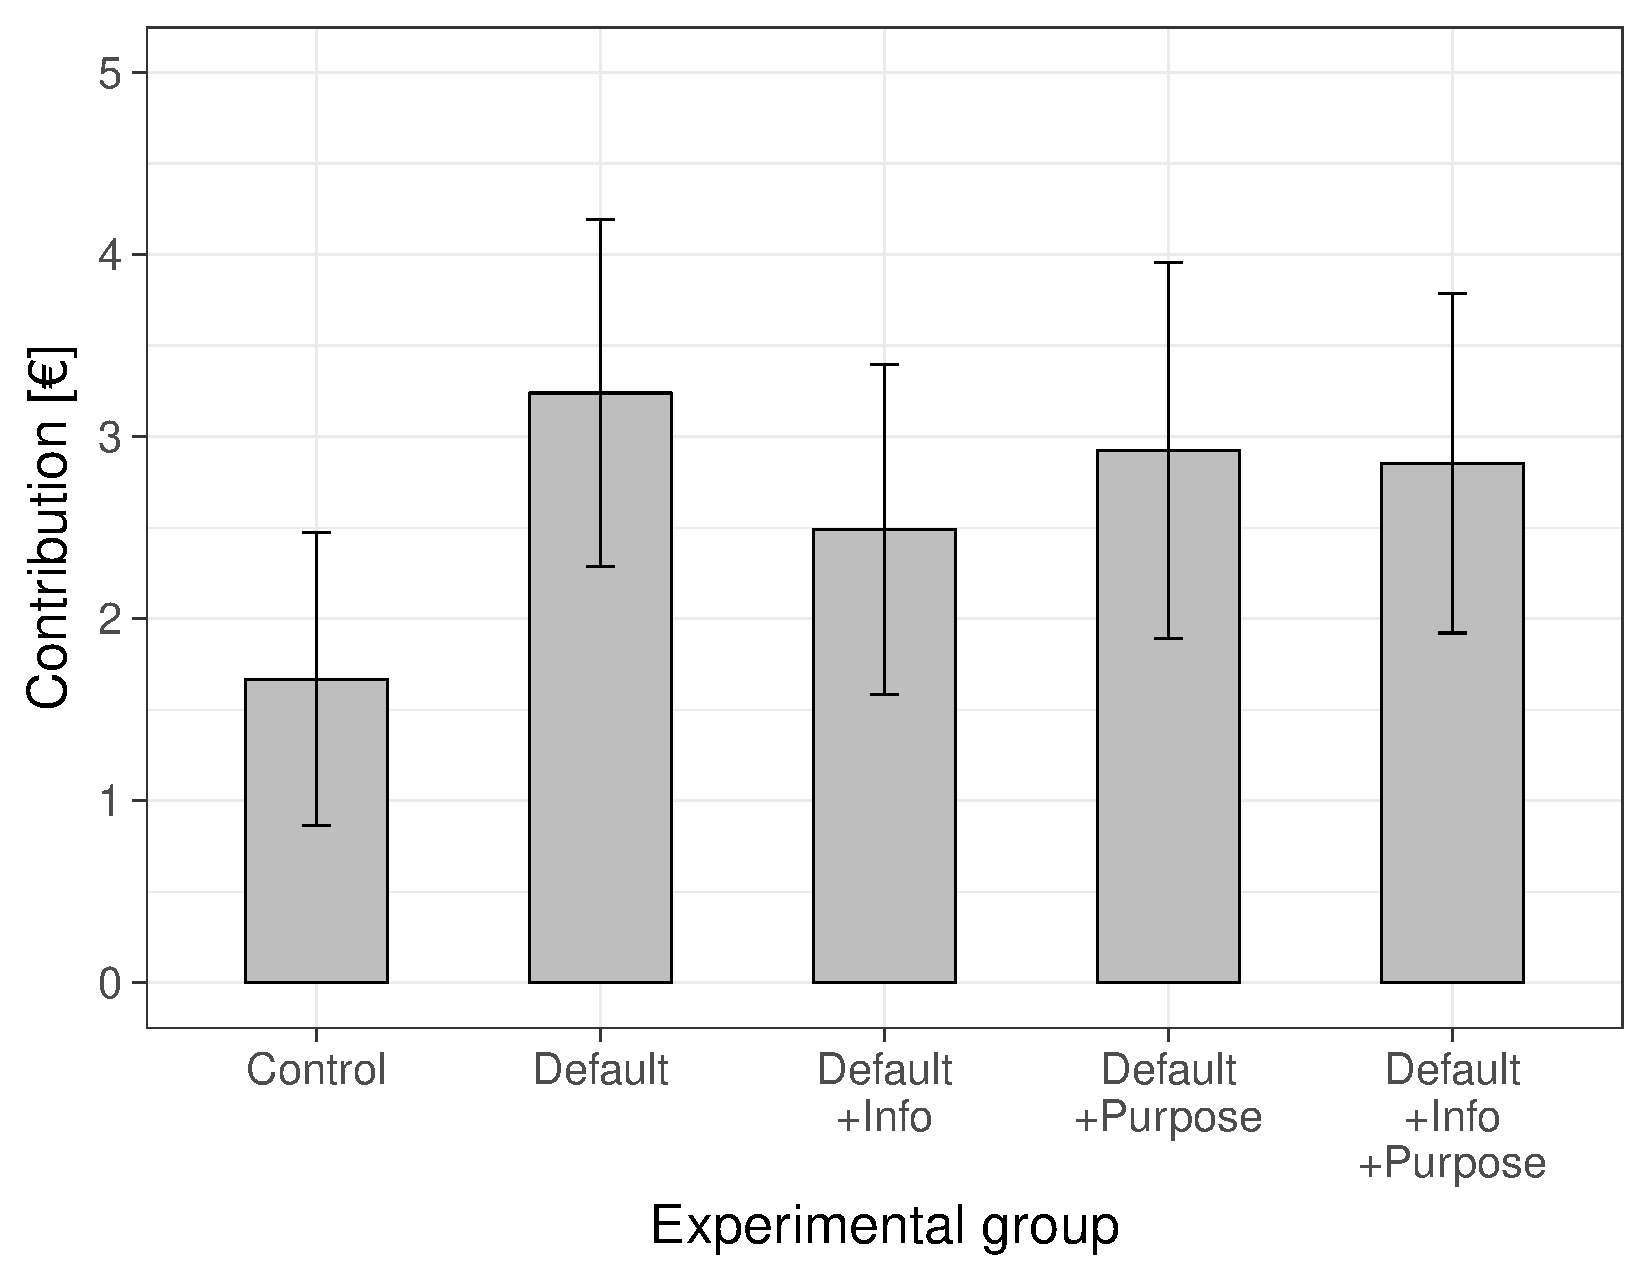
\includegraphics[page=1,width=0.95\textwidth]{Figure1}
  \label{fig1}
  \floatfoot{Notes: Error bars represent 95\% confidence intervals.}
  \end{tabular}
\end{figure}

We use non-parametric tests because we identified outliers, and Shapiro-Wilk normality tests reject the hypothesis that contributions, as well as distances to the default value, are normally distributed (W = 0.806, p = 0.00 for contributions; W = 0.819, p = 0.00 for distances). This is caused primarily by a large amount of zero contributions compared to other possible values (see Figure~\ref{figb4} in \ref{appb}).

Testing H1 with a Mann-Whitney test rejects the null hypothesis of equal contributions at 5\% significance between Control vs. Default (W = 707.5, p = 0.007), Control vs. Default+Purpose (W = 642, p = 0.028), and Control vs. Default+Info+Purpose (W = 687, p = 0.033). We reject H1 in case of a mere default, as well as in case of a default accompanied by its purpose for all outcome variables. For reasons of brevity we will only report statistics for tests of equal contributions, and include all remaining p-values in Tables ~\ref{tabb7} - ~\ref{tabb10}, in~\ref{appb}. In case of a default with information on its potential influence, the difference of contributions (W = 769.5, p = 0.084), distances to the default value, as well as the fraction of subjects contributing are only marginally significant at 10\%. We do not reject the hypothesis that subjects in the Default+Info group picked the default value as often as subjects in the control group did. In case of a default accompanied by both types of transparency, differences to the control group are significant for the remaining outcome variables except for the fraction of subjects donating.

Overall, we find evidence for H1, i.e. that there is a default- and pull-effect. However, evidence is limited for a default combined with information on its potential influence on behavior.

The pull-effect becomes tangible when looking at Table~\ref{tab2}. More than half of the participants in the control group contributed zero, with no contributions between 6 Euro and 9 Euro. In all treatment groups, the fraction of subjects that contributed nothing is lower, and more subjects chose the default value than in the control group. Together with findings outlined above, this suggests that an overall increase of average contributions in the Default, as well as Default+Purpose groups is partially due to an increase in the fraction of subjects that contributed, as well as a higher fraction of subjects that chose the default, or values near the default. In the Default+Info group, we find a marginally significant increase in the extensive margin, whereas in the Default+Info+Purpose group we find a higher fraction of people picking the default value.

To check robustness of the default effect we focus on contributions as an outcome variable in regression. We begin with a restricted model limited to the treatment variable, then add a dummy variable indicating that subjects perceive climate protection to be (very) important, and proceed to add other relevant covariates (Table~\ref{tab3}). The reason we add importance to protect the climate separately is that a Chi\textsuperscript{2}-Test rejects the hypothesis that subjects are equally distributed among the treatment groups with respect to this variable. The test is marginally significant for Control vs. Default ($\chi$\textsuperscript{2}(1) = 3.503, p = 0.061), and for Control vs. Default+Info ($\chi$\textsuperscript{2}(1) = 3.666, p = 0.056).

\begin{table}[htbp]
  \centering
  \begin{adjustbox}{max width=\textwidth}
  \caption{Descriptive statistics of covariates}
    \label{tab3}%
    \begin{tabular}{lcccccc}
    \toprule
    \toprule
          & \multicolumn{6}{c}{Variable and respective statistic} \\
\cmidrule{2-7}          & \multicolumn{2}{c}{\multirow{3}[2]{*}{Age}} & Gender & Impor- & No exp. & EUETS \\
          & \multicolumn{2}{c}{} & \multirow{2}[1]{*}{(Male)} & tance & Exp-  & not \\
          & \multicolumn{2}{c}{} &       & of CP & erience & effective \\
\cmidrule{2-7}    Experimental group & Mean  & SD    & Mean    & Mean    & Mean    & Mean  \\
    \midrule
    Control & 21.8  & 3.1     & 60    & 57.8  & 31.1  & 57.8 \\
    Default & 22    & 2.8     & 60.9  & 78.3  & 30.4  & 60.9 \\
    Default+Info & 22    & 3     & 51.2  & 79.1  & 20.9  & 53.5 \\
    Default+Purpose & 22.3  & 4.7     & 53.8  & 63.4  & 19.5  & 58.5 \\
    Default+Info+Purpose & 22.7  & 3.7     & 58.5  & 51.3  & 20.5  & 64.1 \\
    \bottomrule
    \bottomrule
    \end{tabular}%
    \end{adjustbox}
\end{table}%


By controlling for this variable we ensure that estimates of treatment effects are not conditionally biased. In theory, since covariates come from a questionnaire that is taken by subjects after being exposed to treatments, there is a risk of the respective manipulations being the reason for the differences in importance-ratings. However, we argue that, in case of endogeneity, we would expect this difference also to be significant for the remaining two treatment groups. This is not the case both for comparisons of Control vs. Default+Purpose ($\chi$\textsuperscript{2}(1) = 0.142, p = 0.706) and Control vs. Default+Info+Purpose ($\chi$\textsuperscript{2}(1) = 0.098, p = 0.754).\footnote{Additionally, calculating VIFs for independent variables of the full regression model indicates that multicollinearity is not an issue, with the largest VIF being lower than 10. Furthermore, a Durbin-Wu-Hausman test suggests that endogeneity of Importance of CP is not an issue.} We therefore judge controlling for perceived importance of climate protection as an adequate mean to estimate unbiased treatment effects.

Regarding Tobit models in Table~\ref{tab4}, un-restricted model (3) includes all covariates, i.e. rating of the importance of climate protection, gender, age, no previous experience with experiments, and judgment of buying emission licenses from the EU ETS as an ineffective tool for climate protection. The Tobit model accounts for left-censored contributions. This means we assume that at least some subjects would choose to take from instead of contribute to the public good. This assumption is common in dictator-games and empirically valid \citep{Engel.2011}.

\begin{table}[htbp]\centering
\begin{adjustbox}{max width=\textwidth}
\def\sym#1{\ifmmode^{#1}\else\(^{#1}\)\fi}
\caption{Stepwise Tobit-Regression\label{tab4}}
\begin{tabular}{l*{3}{c}}
\hline\hline
                    &\multicolumn{1}{c}{(1)}&\multicolumn{1}{c}{(2)}&\multicolumn{1}{c}{(3)}\\
                    &\multicolumn{1}{c}{Con.}&\multicolumn{1}{c}{Con.}&\multicolumn{1}{c}{Con.}\\
\hline
               &                     &                     &                     \\
Default             &       2.706\sym{**} &       2.229\sym{*}  &       2.363\sym{**} \\
                    &     (0.962)         &     (0.938)         &     (0.892)         \\
Default+Info        &       1.703\sym{x}  &       1.233         &       1.065         \\
                    &     (0.983)         &     (0.977)         &     (0.898)         \\
Default+Purpose     &       2.307\sym{*}  &       2.510\sym{*}  &       2.518\sym{**} \\
                    &     (1.007)         &     (0.984)         &     (0.910)         \\
Default+Info+Purpose&       2.058\sym{*}  &       1.863\sym{x}  &       1.946\sym{*}  \\
                    &     (0.996)         &     (0.951)         &     (0.913)         \\
Importance of CP       &                     &       2.485\sym{***}&       2.166\sym{**} \\
                    &                     &     (0.673)         &     (0.660)         \\
Gender (Male=1)                &                     &                     &      -1.659\sym{**} \\
                    &                     &                     &     (0.551)         \\
Age                 &                     &                     &     -0.0518         \\
                    &                     &                     &    (0.0816)         \\
No exp. Experience        &                     &                     &      -0.345         \\
                    &                     &                     &     (0.673)         \\
EUETS not effective &                     &                     &      -2.400\sym{***}\\
                    &                     &                     &     (0.569)         \\
Constant            &      -0.129         &      -1.595\sym{x}  &       2.358         \\
                    &     (0.737)         &     (0.824)         &     (1.965)         \\
\hline
Sigma               &                     &                     &                     \\
Constant            &       4.160\sym{***}&       4.020\sym{***}&       3.777\sym{***}\\
                    &     (0.250)         &     (0.254)         &     (0.229)         \\
\hline
Observations        &         214         &         214         &         214         \\
\hline\hline
\multicolumn{4}{l}{\footnotesize Robust standard errors in parentheses}\\
\multicolumn{4}{l}{\footnotesize \sym{x} \(p<0.10\), \sym{*} \(p<0.05\), \sym{**} \(p<0.01\), \sym{***} \(p<0.001\)}\\
\end{tabular}
\end{adjustbox}
\end{table}

Model (1) predicts that a mere default, a default plus its purpose, as well as a default plus both types of transparency lead to higher average contributions compared to no default. The effect of Default+Info is only marginally significant. When controlling for subjects' perception of the importance of climate protection in model (2), all coefficients, except that of Default+Purpose, decrease. This results in non-significance for Default+Info. As argued above, we judge these coefficients to be conditionally unbiased, and therefore more appropriate in order to estimate treatment effects. The positive effect of \textit{Importance of CP} on the outcome is highly significant. A likelihood-ratio test suggests that the un-restricted model fits the data significantly better ($\chi$\textsuperscript{2}(1) = 14.47, p = 0.00). Controlling for additional covariates increases precision of the estimated average treatment effects. A likelihood-ratio test suggests that un-restricted model (3) fits the data significantly better than restricted model (2) ($\chi$\textsuperscript{2}(4) = 26.34, p = 0.00).

Based on the full model, a default, as well as a default supplemented by its purpose, increase average contributions to the public good by 2.36 Euro and 2.52 Euro, respectively, compared to no default. A default with full transparency increases contributions by 1.95 Euro. \\

%%\hfill\begin{minipage}{\dimexpr\textwidth-1cm}
F1: There is a default effect on contributions for a default, a default with added purpose, as well as for a default with both types of transparency. \\
%\end{minipage}

\subsection{Influence of transparency on default effectiveness}
We proceed testing H2 $-$ H4. A Kruskal-Wallis test for equal contributions in the treatment groups is insignificant (H(3) = 1.117, p = 0.773). So are respective pairwise comparisons with Dunn's test (not reported). Contributions in the treatment groups do not significantly differ from each other. The same holds for distances to the default value (H(3) = 1.459, p = 0.692), the fraction of subjects choosing to contribute ($\chi$\textsuperscript{2}(3) = 0.860, p = 0.835, Chi\textsuperscript{2}-Test), as well as the fraction of subjects choosing the default value (p = 0.346, Fisher's exact test). Consequently, for neither of the four outcome variables we find significance in the differences suggested by H2, i.e. between Default and Default+Info; H3, i.e. between Default+Purpose and Default; and H4, i.e. between Default+Purpose, Default+Info+Purpose, and Default+Info, even though effects go into the hypothesized direction (Table~\ref{tab2}).
As above, we augment our analysis by focusing on contributions in stepwise Tobit-regression (Table~\ref{tab4}). In un-restricted model (3), an omnibus Wald-test for equality of parameter estimates for Default, Default+Info, Default+Purpose, and Default+Info+Purpose does not allow us to reject the null hypothesis at any conventional significance level (F(3, 205) = 1.11, p = 0.344). The same holds for restricted models. We find no evidence of unequal contributions in the treatment groups. Consequently, we find no evidence that transparency significantly reduces contributions\footnote{We plot estimated treatment-effects of un-restricted regression models in~\ref{appb} (Figures~\ref{figb5},~\ref{figb6}, and~\ref{figb7}). Although we conducted a power analysis prior to the experiment, we agree with \cite{Colegrave.2003} that confidence intervals are more informative to insignificant tests.}. \\

F2: Informing participants that the default may have an influence on their decision does not significantly decrease contributions compared to when they are not informed.\\

F3: Informing participants about the default's purpose does not significantly increase contributions compared to when they are not informed.\\

F4: Informing participants that the default may have an influence on their decision, as well as of the default's purpose does not decrease or increase contributions, compared to the other types of transparency (including no transparency at all).\\

Regarding the additional covariates, \textit{Gender} and \textit{EUETS not effective} are significant. Being male, as well as judging the EU ETS as not effective to protect the climate, decrease average contributions. The former finding is consistent with evidence from dictator games \citep{Engel.2011}. Findings on gender differences in public good games are ambiguous, however \citep{Croson.2009}. In the context of real contributions to climate protection, evidence by \cite{Diederich.2014}, while suggesting that female subjects are less indifferent to climate protection, do not support a higher willingness to pay for emission certificates of women. Findings with respect to age somewhat align with those of \cite{Borghans.2015} who find, in a less restricted sample, that the default effect does vary with age. However, at around 22 years (the mean of our sample) they find a relatively large default effect. This may explain why we find a default effect, but no effect of age.

\subsection{Psychological reactance and transparency}
In order to find out whether reactions to different types of transparency can be explained by psychological reactance, we create an index for each of the two state reactance-categories, i.e. for the perceived threat to freedom and the anger-category.\footnote{We constructed a dummy-variable, which is equal to 1 when the subject "agreed" or "strongly agreed", resp. replied with "to some extent" or "very" to the respective statements, for each item (see~\ref{appc}). Then, we added the respective dummies in each category, to form two indexes, each ranging from zero to four. Findings are consistent for when both dependent variables are included as (un-weighted) factor-based scores in linear OLS-regression.}

We model the log odds of subjects being in a higher level of each of both ordinal indexes on all explanatory variables used above (Table~\ref{tab5}). Note that this regression excludes observations from the control group since subjects in this group were not presented with the default option.

\begin{table}[htbp]\centering
\begin{adjustbox}{max width=\textwidth}
\def\sym#1{\ifmmode^{#1}\else\(^{#1}\)\fi}
\caption{Ordered logistic model of state reactance\label{tab5}}
\begin{tabular}{l*{2}{c}}
\hline\hline
                    &\multicolumn{1}{c}{(4)}&\multicolumn{1}{c}{(5)}\\
                    &\multicolumn{1}{c}{ThreatToFreedom}&\multicolumn{1}{c}{Anger}\\
\hline
                &                     &                     \\
Default+Info        &      0.0933         &      -0.342         \\
                    &     (0.401)         &     (0.395)         \\
Default+Purpose     &    -0.00976         &     -0.0155         \\
                    &     (0.456)         &     (0.454)         \\
Default+Info+Purpose&     -0.0443         &      -0.588         \\
                    &     (0.357)         &     (0.478)         \\
Importance of CP       &      -0.129         &      -0.349         \\
                    &     (0.307)         &     (0.352)         \\
Gender (Male=1)                &      -0.142         &      -0.199         \\
                    &     (0.303)         &     (0.328)         \\
Age                 &     -0.0368         &     -0.0912\sym{*}  \\
                    &    (0.0373)         &    (0.0422)         \\
No ex. Experience        &     0.00944         &      0.0802         \\
                    &     (0.303)         &     (0.420)         \\
EUETS not effective &     -0.0180         &      0.0365         \\
                    &     (0.321)         &     (0.331)         \\
\hline
Cut1                &                     &                     \\
Constant            &      -2.703\sym{**} &      -2.098\sym{x}  \\
                    &     (0.950)         &     (1.111)         \\
\hline
Cut2                &                     &                     \\
Constant            &      -1.918\sym{*}  &      -1.478         \\
                    &     (0.917)         &     (1.126)         \\
\hline
Cut3                &                     &                     \\
Constant            &      -0.729         &      -0.712         \\
                    &     (0.890)         &     (1.133)         \\
\hline
Cut4                &                     &                     \\
Constant            &       0.523         &      -0.123         \\
                    &     (0.875)         &     (1.156)         \\
\hline
Observations        &         169         &         169         \\
\hline\hline
\multicolumn{3}{l}{\footnotesize Robust standard errors in parentheses}\\
\multicolumn{3}{l}{\footnotesize \sym{x} \(p<0.10\), \sym{*} \(p<0.05\), \sym{**} \(p<0.01\), \sym{***} \(p<0.001\)}\\
\end{tabular}
\end{adjustbox}
\end{table}


None of the coefficients modeling treatment effects are significant.\footnote{This finding is consistent with non-parametric tests for differences of individual items of the scales (not reported).} \\

%%\hfill\begin{minipage}{\dimexpr\textwidth-1cm}
F5: Combining the default with information about its potential behavioral influence does not increase participants' experience of state reactance. \\
%%\end{minipage}

We find a significant negative influence of age on experienced anger triggered by the default value. The finding that experiencing negative emotions decreases with age is known in the literature \citep[e.g.][]{Charles.2001}.

To further test if reactions towards the combination of a default value with different types of transparency can be explained by psychological reactance, we measured subjects' proneness to experience psychological reactance. To create an index for trait reactance, we proceeded similarly to the case of state reactance.\footnote{We constructed dummy variables for each of the 14 items of the scale, which are equal to 1 when the subject responded with "Agree" or "Strongly agree" to the respective question, 0 otherwise. We then added the dummies for each subject to create the index, which ranges from zero to 14. Findings are consistent for trait reactance included as a (un-weighted) factor-based score.}

\begin{table}[htbp]\centering
\begin{adjustbox}{max width=\textwidth}
\def\sym#1{\ifmmode^{#1}\else\(^{#1}\)\fi}
\caption{Stepwise Tobit-models with interaction term \label{tab6}}
\begin{tabular}{l*{3}{c}}
\hline\hline
                    &\multicolumn{1}{c}{(6)}&\multicolumn{1}{c}{(7)}&\multicolumn{1}{c}{(8)}\\
                    &\multicolumn{1}{c}{Con.}&\multicolumn{1}{c}{Con.}&\multicolumn{1}{c}{Con.}\\
\hline
               &                     &                     &                     \\
Default+Info        &      -0.914         &      -0.914         &      -1.217         \\
                    &     (0.880)         &     (0.868)         &     (0.832)         \\
Default+Purpose     &      -0.448         &       0.204         &       0.115         \\
                    &     (0.902)         &     (0.916)         &     (0.889)         \\
Default+Info+Purpose&      -0.648         &      -0.381         &      -0.462         \\
                    &     (0.907)         &     (0.849)         &     (0.858)         \\
Reactance          &     -0.0743         &      -0.119         &     -0.0397         \\
                    &     (0.220)         &     (0.211)         &     (0.210)         \\
Default+Info $\times$ Reactance&      -0.249         &      -0.219         &      -0.193         \\
                    &     (0.276)         &     (0.269)         &     (0.254)         \\
Default+Purpose $\times$ Reactance&       0.166         &       0.227         &      0.0687         \\
                    &     (0.338)         &     (0.340)         &     (0.316)         \\
Default+Info+Purpose $\times$ Reactance&      0.0502         &      0.0597         &      -0.111         \\
                    &     (0.298)         &     (0.279)         &     (0.278)         \\
Importance of CP       &                     &       2.431\sym{**} &       2.120\sym{**} \\
                    &                     &     (0.741)         &     (0.718)         \\
Gender (Male=1)                &                     &                     &      -1.597\sym{*}  \\
                    &                     &                     &     (0.648)         \\
Age                 &                     &                     &      0.0231         \\
                    &                     &                     &    (0.0775)         \\
No exp. Experience        &                     &                     &      -0.485         \\
                    &                     &                     &     (0.735)         \\
EUETS not effective &                     &                     &      -2.258\sym{***}\\
                    &                     &                     &     (0.593)         \\
Constant            &       2.615\sym{***}&       0.721         &       3.112\sym{x}  \\
                    &     (0.616)         &     (0.844)         &     (1.846)         \\
\hline
Sigma               &                     &                     &                     \\
Constant            &       4.022\sym{***}&       3.890\sym{***}&       3.686\sym{***}\\
                    &     (0.244)         &     (0.246)         &     (0.232)         \\
\hline
Observations        &         169         &         169         &         169         \\
\hline\hline
\multicolumn{4}{l}{\footnotesize Robust standard errors in parentheses}\\
\multicolumn{4}{l}{\footnotesize \sym{x} \(p<0.10\), \sym{*} \(p<0.05\), \sym{**} \(p<0.01\), \sym{***} \(p<0.001\)}\\
\end{tabular}
\end{adjustbox}
\end{table}

Specifically, we test whether subjects' reactions towards different types of transparency accompanying the default differ depending on subjects' trait reactance. Therefore, we run regressions with an interaction term of treatment variable and trait reactance index. The latter is centered on the mean, so that treatment-main-effects are meaningful (Table~\ref{tab6}). Note that this regression excludes observations from the control group. For reasons of brevity, we focus on the main effects of trait reactance, as well as on interaction-effects.

As in previous Tobit models, model (7) fits the data better than model (6) ($\chi$\textsuperscript{2}(1) = 11.47, p = 0.00), and model (8) fits the data better than model (7) ($\chi$\textsuperscript{2}(4) = 19.71, p = 0.00).We find no significant main effect of trait reactance, nor do we find that the different types of transparency and the trait reactance index interact significantly for any of the three model-specifications. In other words, there is no evidence that the effect of different types of transparency on average contributions is conditional on subjects' trait reactance. \\

%%\hfill\begin{minipage}{\dimexpr\textwidth-1cm}
F6: The influence of information on the default effect does not depend on the level of trait reactance of participants. \\
%%\end{minipage}

Both approaches that are linking different types of transparency of a default to psychological reactance suggest that subjects neither perceive a default value differently based on the type of transparency accompanying it, nor does their inherent propensity to show psychological reactance change the way they react to these different types of transparency.

\section{Discussion and conclusion}
This study contributes to the discussion of nudges and transparency by providing empirical evidence. Despite the widespread application of nudges, some people are concerned of the potentially manipulative nature of behavioral interventions. In democratic societies, public authorities are expected to be transparent with regard to their actions and intentions. Therefore, covertly 'exploiting' people's psychological biases might have an impact on perceived legitimacy, and ultimately effectiveness of such policies. The most straightforward solution to this problem is to instruct policy-makers to disclose information regarding the potential influence of the nudge, and its purpose. However, this suggestion raises the concern that nudges will no longer be effective. As expressed by \cite{Bovens.2009}, nudges "work best in the dark".

The results of this study suggest that this concern might be overstated. Our experiment provides evidence that defaults increase contributions to climate protection even when complemented by a disclosure regarding the potential influence of the default and its purpose, or just its purpose. However, it is not clear whether informing subjects only of the potential influence of the default has an impact on contributions. Furthermore, we find no evidence that additional information on the potential behavioral influence and/or purpose of the default triggers psychological reactance. Likewise, we find no evidence that subjects differing in their proneness to experience reactance also differ in how they react towards the default with additional information.

These findings suggest that despite the initial concern over the inhibiting influence of transparency, nudges in the form of defaults can be transparent and at the same time effective. However, the type of transparency might matter. In order to preserve the effect of defaults and increase the legitimacy of behaviorally informed policies, policy makers should be transparent about their motives. The motive itself and how it is perceived by the decision maker has been found to matter for advice \citep{Kuang.2007}, and might also matter for defaults, as well as nudges in general.

Our findings support and add to previous evidence on the influence of transparency. \cite{Loewenstein.2015} and \cite{Kroese.2016} found that pro-self defaults were effective in health contexts even after disclosing information about them. Our study extends this conclusion to pro-social nudges, a type that is widely used in the context of public policy-making. Moreover, we extend findings by \cite{Steffel.2016} by examining the influence of transparency in a more realistic setting where participants' decisions have an actual consequence for them, and for the environment. Findings are also useful for the private sector and NGOs aiming to include nudges in their inventory to increase contributions to environmental protection, and possibly other public goods, e.g. charity.

Although several recent studies link nudges to psychological reactance, they do so either indirectly, or they deal with hypothetical and attitudinal, instead of behavioral outcomes \citep{Haggag.2014, Arad.2015, Loewenstein.2015, Hedlin.2016}. By measuring both state and trait reactance, we enable a more direct way of assessing the role of psychological reactance in the influence of transparency on the effectiveness of a default value. To our best knowledge, \cite{Goswami.2016} is the only study that assesses the interaction of trait reactance with the size of a default value on behavioral outcomes, i.e. charitable giving. They find no significant interaction effect. On a more general level, our findings, in line with theirs, suggest that psychological reactance plays a lesser or no role with respect to behavioral effects of defaults, and, in our case, transparency.

Further research could evaluate the role of trait reactance on how subjects respond to different types of transparency for different types of nudges, i.e. social norms or framing. Since our experiment has a rather limited amount of subjects, field experiments can establish statistically more powerful findings for interaction effects. Due to a more realistic context, a field experimental approach would also increase external validity. Nevertheless, our experiment is less abstract than a 'regular' laboratory experiment due to the fact that contributions have a real effect on climate protection \cite{Harrison.2004}. The current study focuses on one type of nudge, and a specific context. Further research is needed in order to determine the overall influence of transparency on the effectiveness of nudges. Moreover, results might be context-specific, thus requiring further investigation into pro-social nudges. Delving into the welfare implications of transparency can also become a promising research endeavor \citep{Sunstein.2015}.

Overall, our findings advance the understanding of how nudges in general, and defaults specifically, affect individual behavior with social consequences, and how policy-makers can increase their transparency without limiting their effectiveness.


\section*{Acknowledgments}
We would like to thank Christoph Engel, Olexandr Nikolaychuk, Oliver Kirchkamp, and other participants of the IMPRS Summer School 2015, Jena, for their valuable comments. In addition, we would like to thank the participants of the Behavioural Insights in Research and Policy Making SABE/IAREP Conference 2016, Wageningen, and a guest lecture at the faculty of Governance and Global Affairs, Leiden University, for useful suggestions. For the same reasons we also thank the participants of the 11th Conference on Empirical Legal Studies. We also thank Nieke Elbers and participants of the Empirical Legal Studies Workshop at the University of Amsterdam. We also thank Claudia Schwirplies, Jaroslaw Kantorowicz, and Maximilian Kerk for their help. All possible mistakes remain, however, our own. \\
Funding: This work was supported by the ESL Innovation Program, Erasmus University Rotterdam, Netherlands. Experimental design, analysis and interpretation of data, writing the report, as well as the decision to submit the article for publication were decided on solely by the authors of this paper.


\section*{References}


\bibliographystyle{model5-names}
\bibliography{reflist}

\clearpage

\appendix

\section{Experimental design}
\label{appa}
\textbf{Instructions} \\
Welcome and thank you very much for participating in this experiment.
This experiment is about decision-making. Please read the following instructions carefully. Everything that you need to know in order to participate in this experiment is explained below. If you have any difficulties in understanding these instructions please raise your hand and I will come to you.
Please note that communication between participants is strictly prohibited during the experiment. Communication between participants will lead to the exclusion from the experiment.
The experimental procedure will be as follows.
You will receive 10 Euro. Please decide how much of the 10 Euro you would like to spend on climate protection. You can choose freely how much, if any, you contribute to climate protection (whole numbers between 0-10).
Should you decide to contribute, we will realize your contribution to climate protection by buying and retiring carbon emission licenses from the European Union Emissions Trading System (EU ETS) at the end of the experiment (please read the respective paragraph below for a description). By this, you have the possibility to make a real contribution to climate protection. The rest of the money is your private pay-out that you will receive in cash at the end of the experiment.

After making the decision you will be kindly asked to complete a short questionnaire.
Please note that your decisions in this experiment are anonymous and will not be revealed at any stage to the other participants. (If relevant) a confirmation of the aggregated real payment to the climate protection fund will be sent to all participants at the end of the whole experiment. \\

\textbf{The Climate Protection Fund} \\
If a person wants to protect the climate, emitting climate gases such as CO$_2$ should be avoided. But it is possible to do even more: Individuals can buy and delete emission certificates from the EU Emission Trading System (ETS) through certified organizations and NGOs. By doing so, a private person reduces the amount of CO$_2$ which can be emitted by European industries, protects the environment and ensures that the development of climate-friendly technologies is accelerated.
In this experiment, the participants' contributions to the climate protection fund will be used to buy real carbon dioxide (CO$_2$) emission licenses on the market of the European Union Emissions Trading Scheme (EU ETS) via the website "TheCompensators.org". It is one example of an NGO that allows ordinary people to directly participate in the EU ETS scheme, and where they can make decisions on CO$_2$ reductions.

The following table shows how much kilograms of carbon you reduce with your payment, and how much money you receive for yourself. The far right row indicates the respective amount of reduced CO$_2$ relative to a Dutch citizens' average of 9163 kg of CO$_2$ emitted per year.

\begin{table}[h]
   \centering
   \begin{tabular}{@{}c@{\hspace{.5cm}}c@{}}
       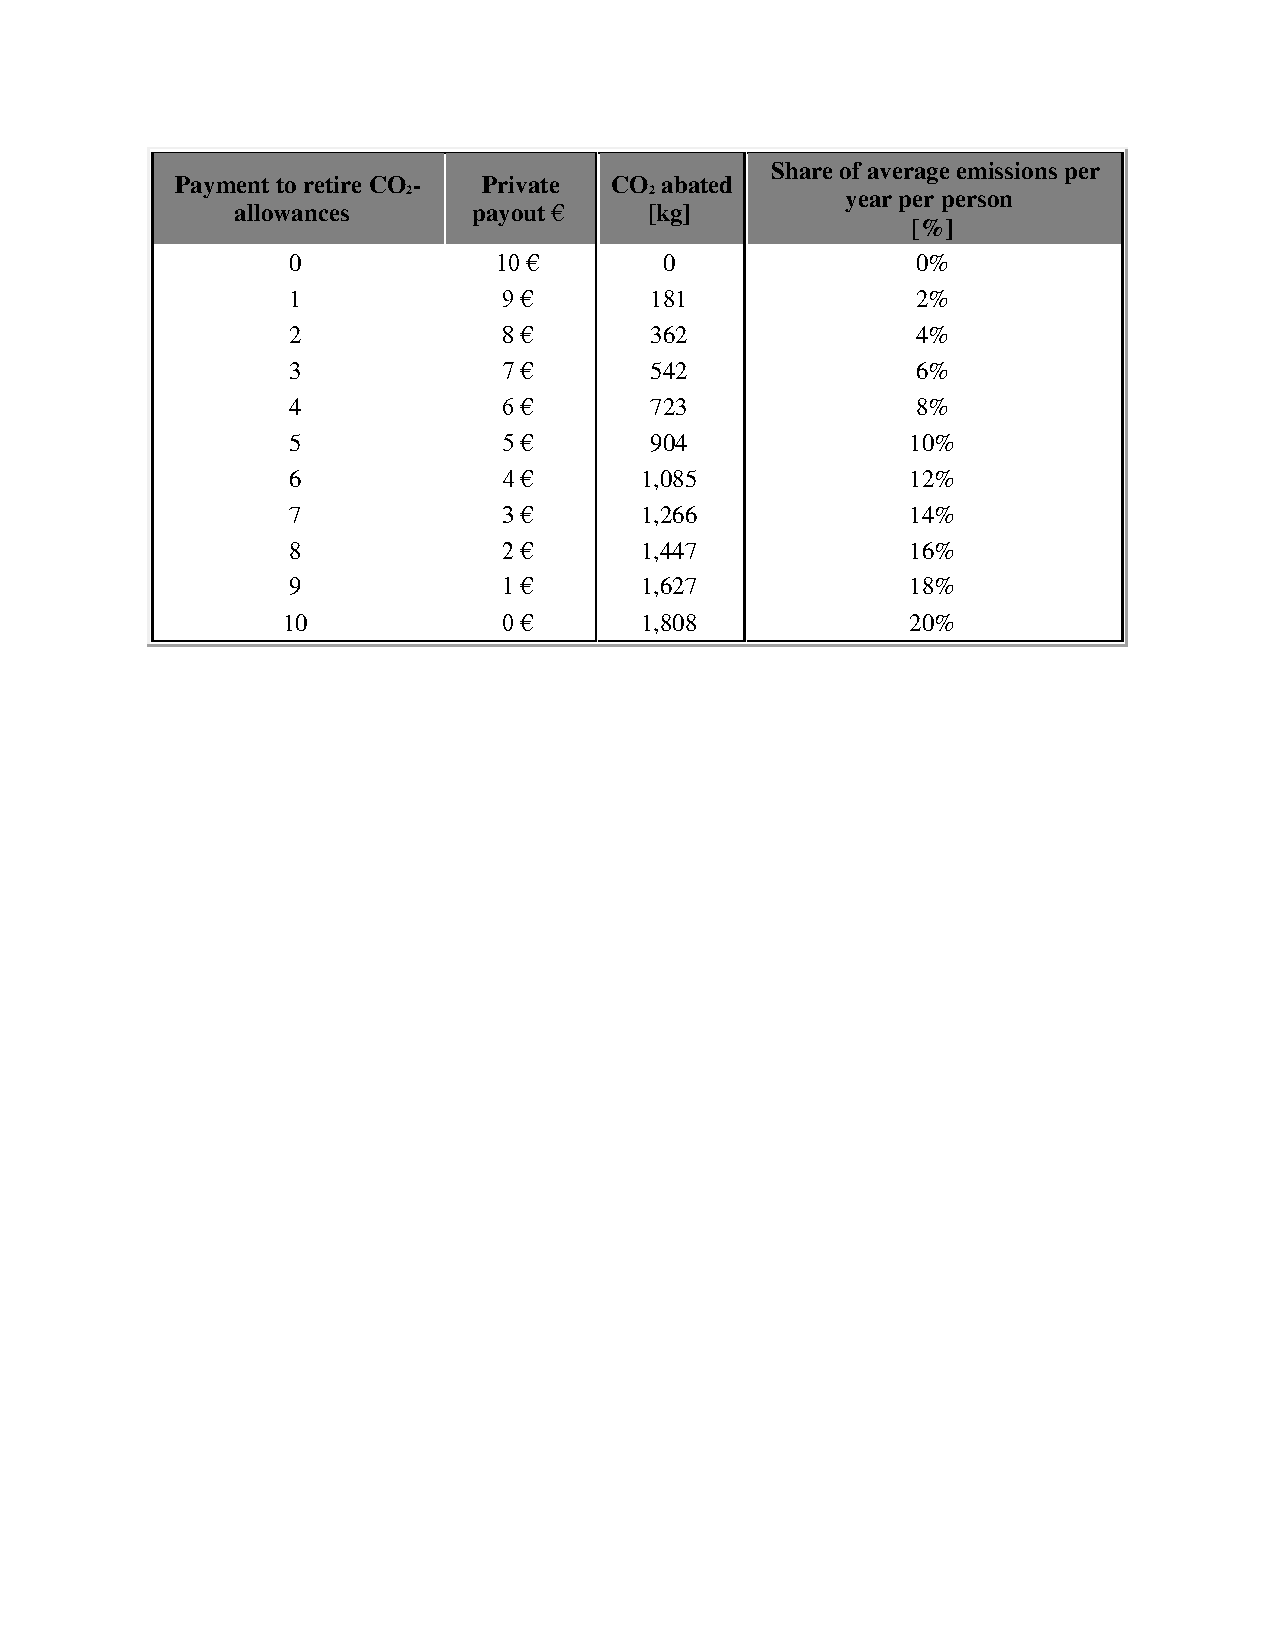
\includegraphics[page=1,width=1\textwidth]{InstructTable}
    \end{tabular}
\end{table}

For example, with a payment of 3 Euro to retire carbon licenses, you retire 542 kg CO$_2$. This corresponds to approximately 6\% of the average emissions per capita per year of a Dutch person. As a private pay-out you get 7 Euro. With a payment of 8 Euro to retire carbon licenses, you retire 1,447 kg CO$_2$. This corresponds to approximately 16\% of the average emissions per capita per year of a Dutch person. As a private pay-out you get 2 Euro.

\begin{figure}[h]
\caption{Experimental screen for Control}
   \centering
   \begin{tabular}{@{}c@{\hspace{.5cm}}c@{}}
       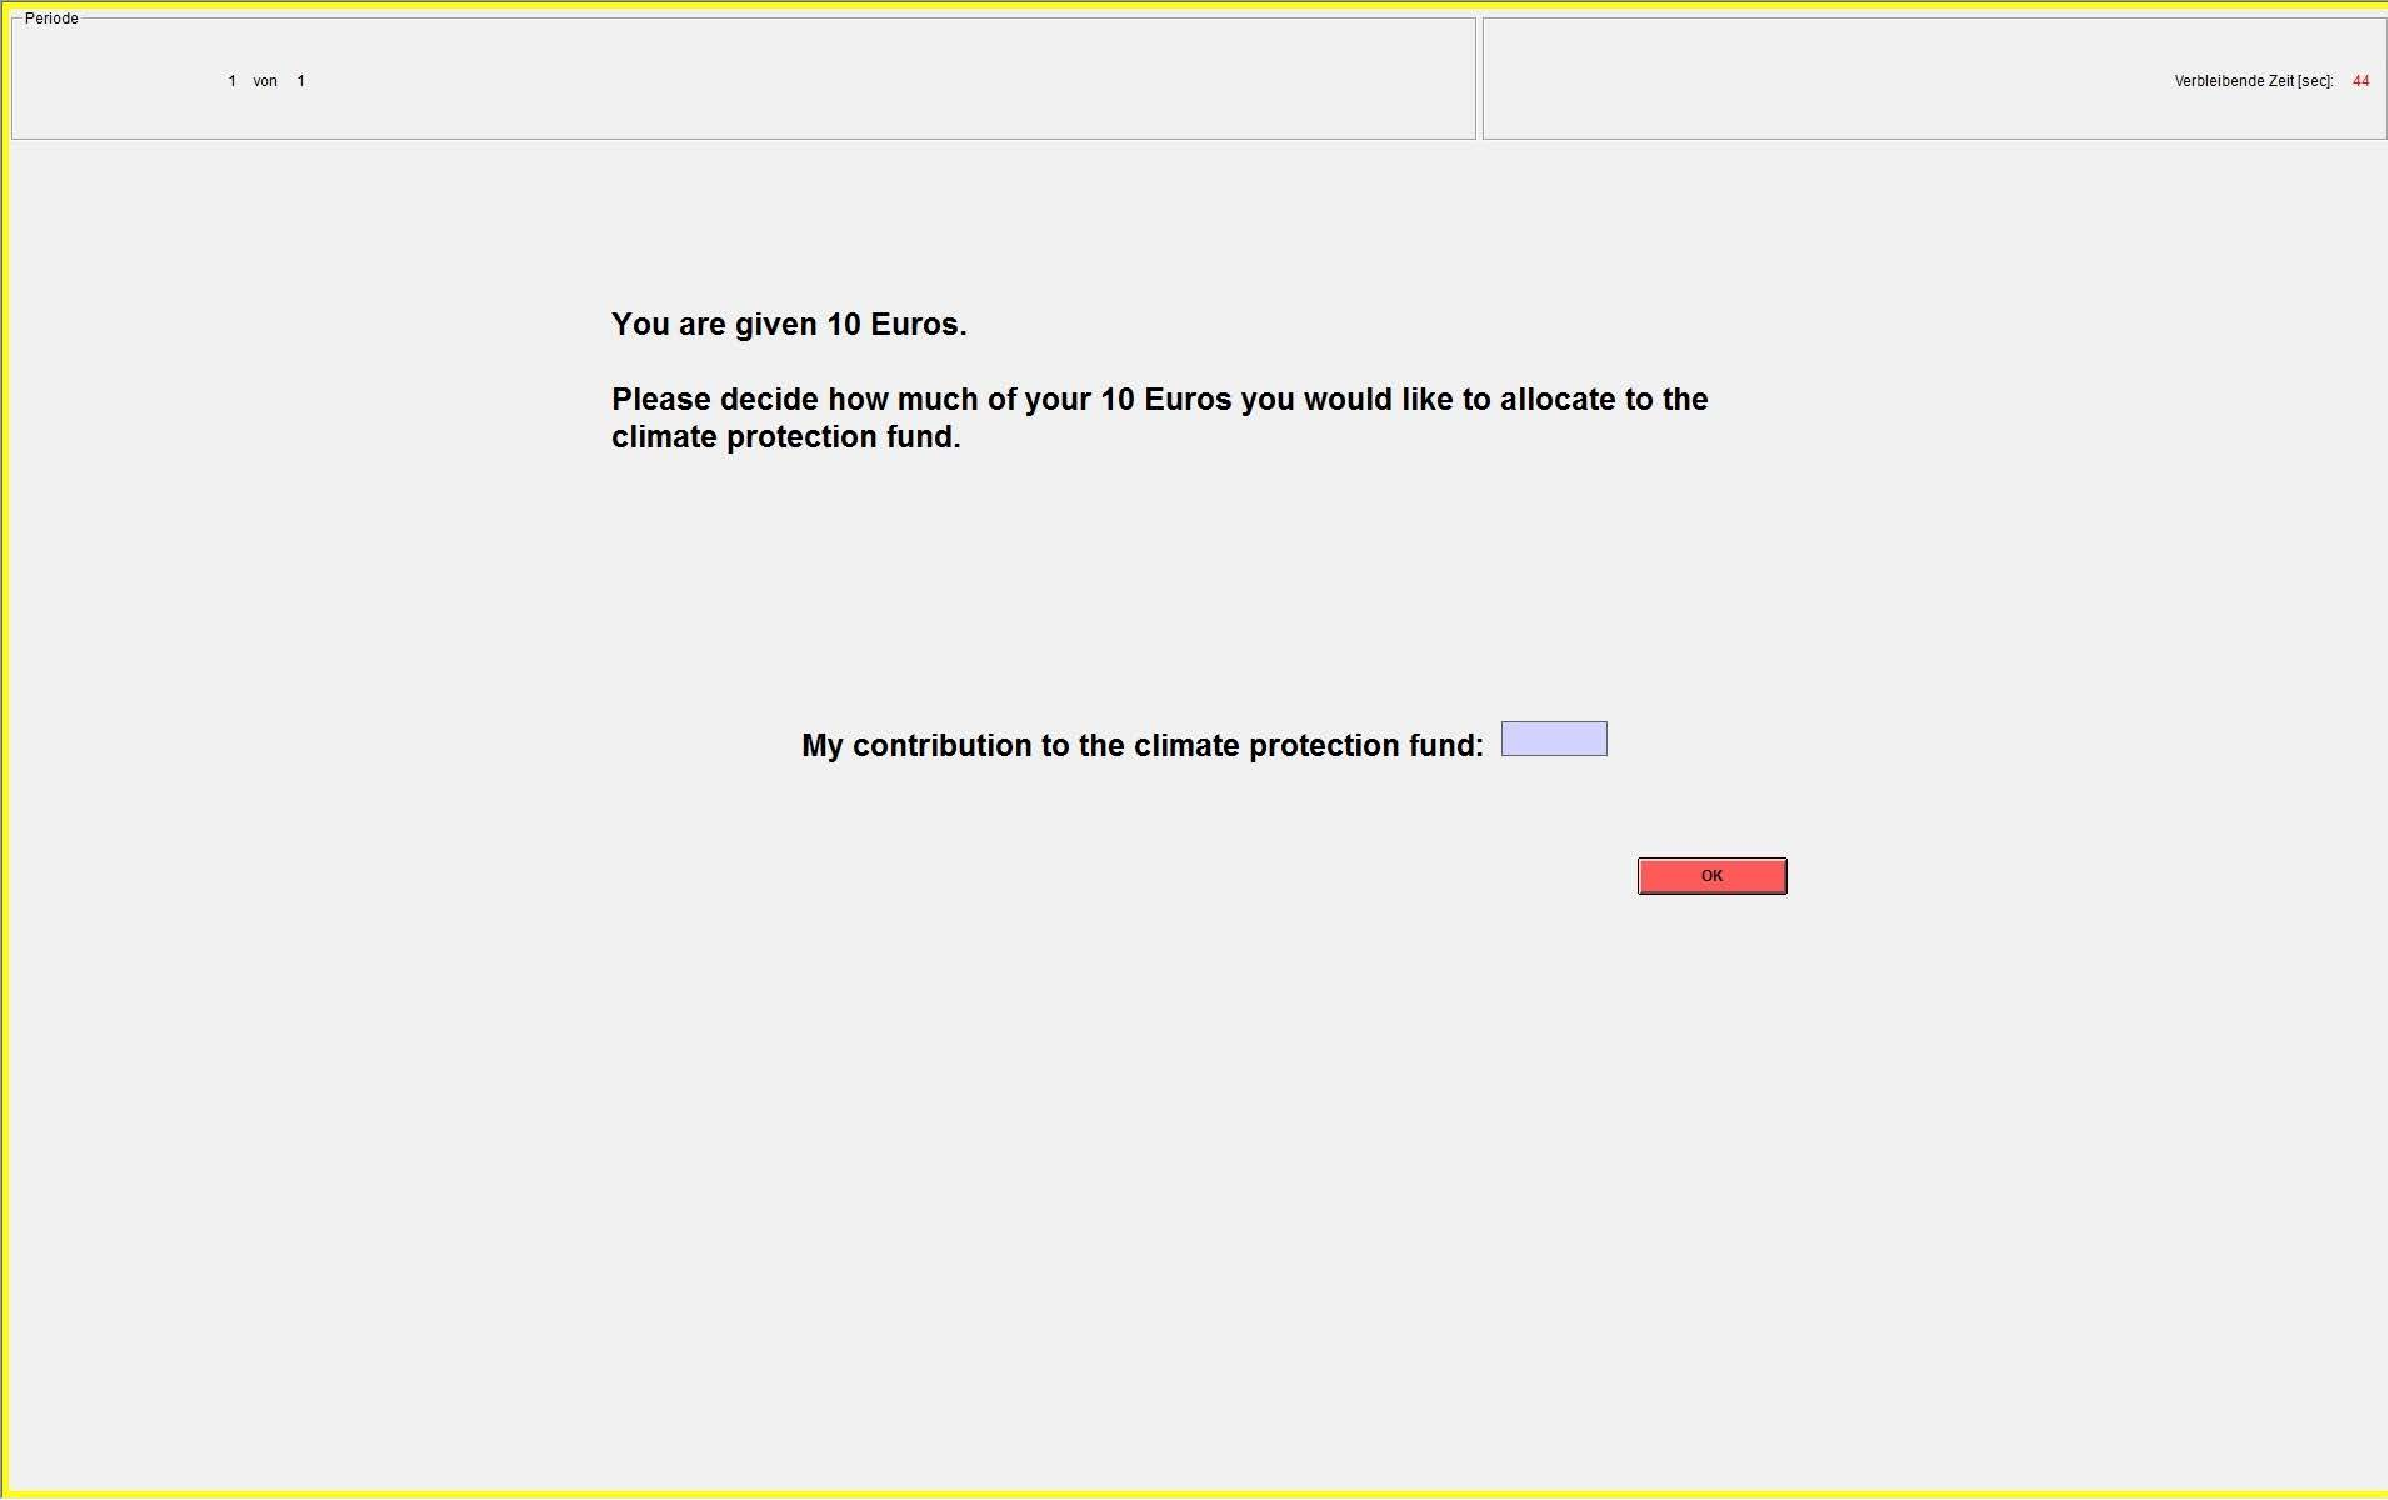
\includegraphics[page=1,width=0.8\textwidth]{FigureA2}
  \label{figa2}
  \end{tabular}
\end{figure}

\begin{figure}[h]
\caption{Experimental screen for Default + transparency}
   \centering
   \begin{tabular}{@{}c@{\hspace{.5cm}}c@{}}
       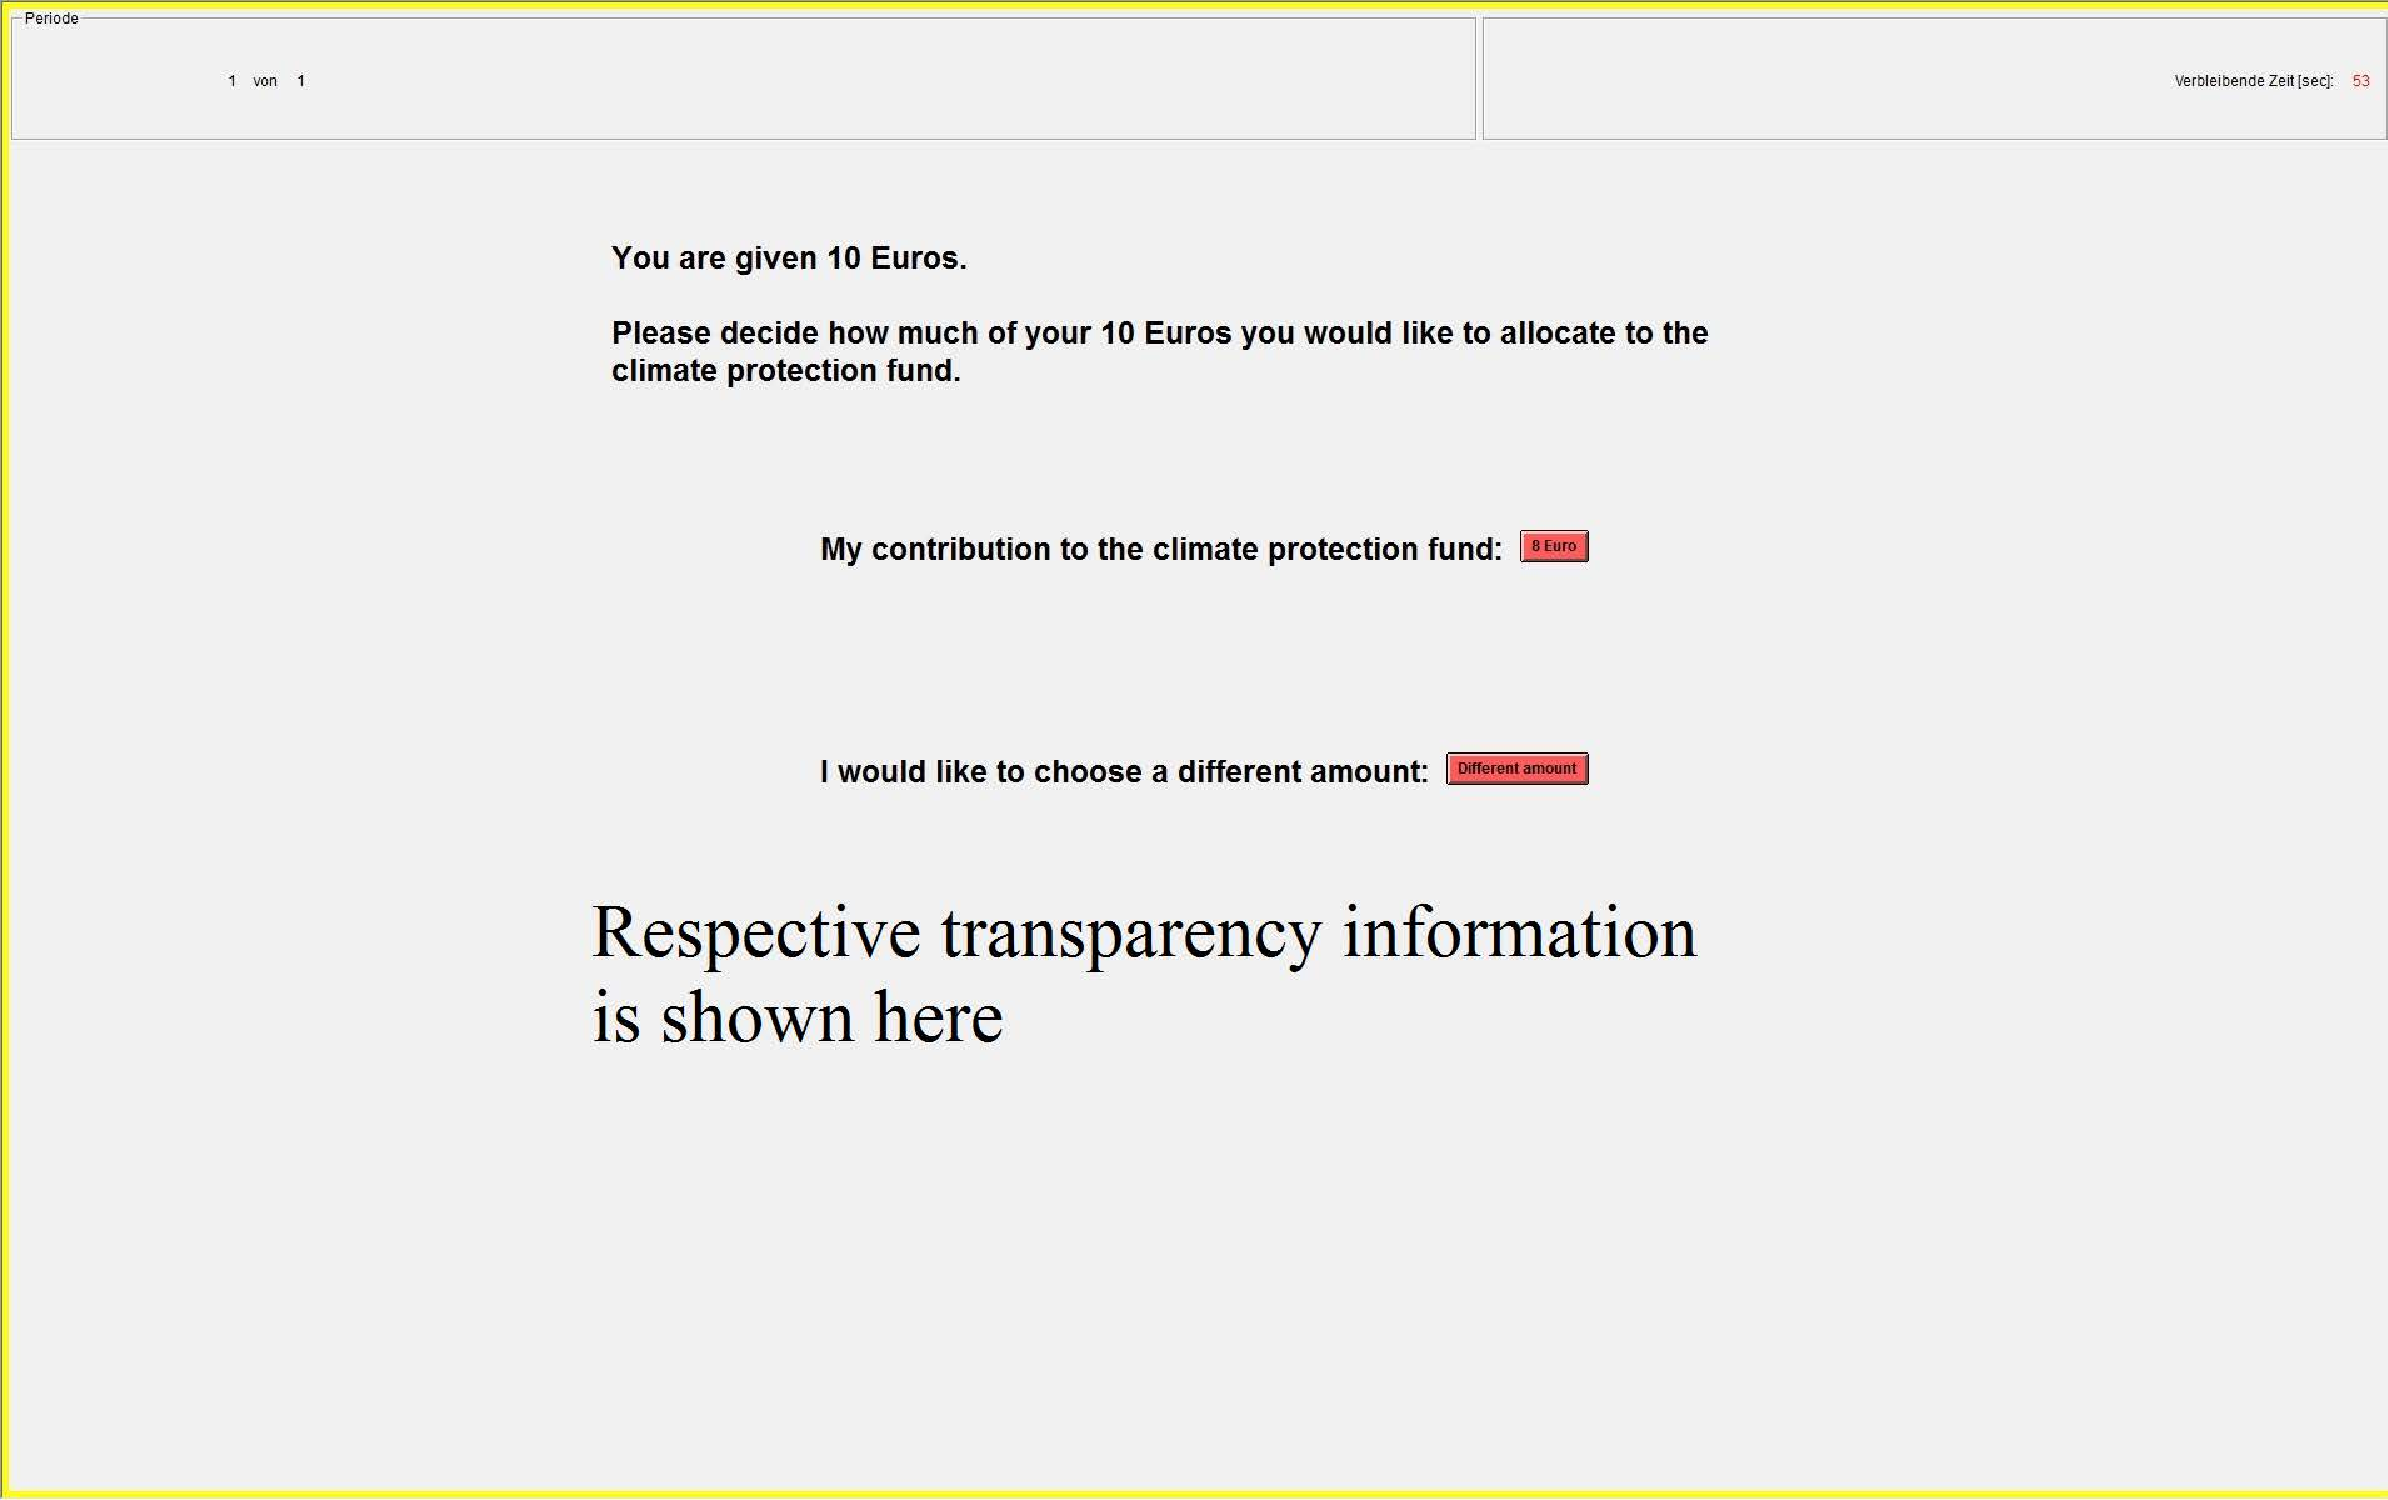
\includegraphics[page=1,width=0.8\textwidth]{FigureA3}
  \label{figa3}
  \end{tabular}
\end{figure}

\clearpage

\section{Statistical analyses}
\label{appb}
\begin{figure}[h]
\caption{Distribution of contributions}
   \centering
   \begin{tabular}{@{}c@{\hspace{.5cm}}c@{}}
       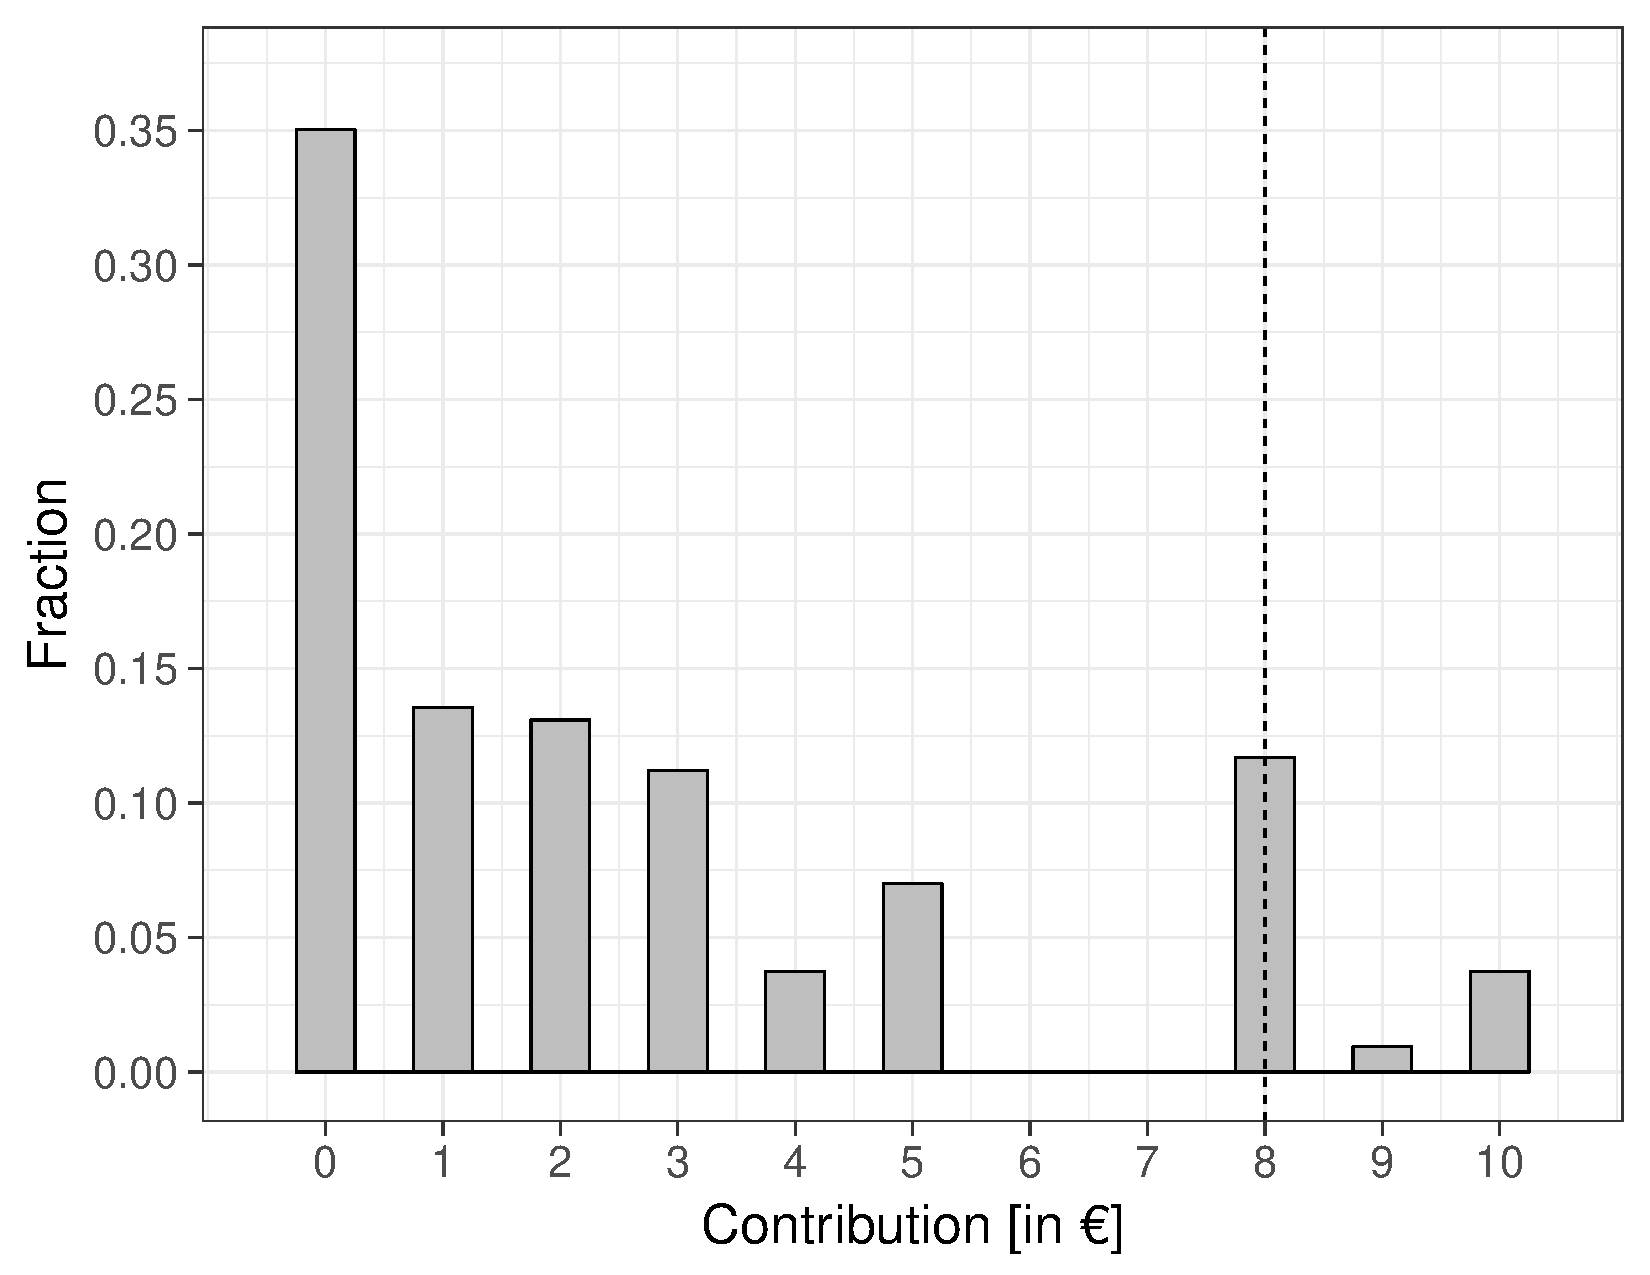
\includegraphics[page=1,width=1\textwidth]{FigureB4}
  \label{figb4}
  \floatfoot{Notes: The dashed line indicates the default value}
  \end{tabular}
\end{figure}


\begin{table}[htbp]
  \centering
  \begin{adjustbox}{max width=\textwidth}
  \caption{P-values for pairwise MW tests of Contribution}
    \label{tabb7}%
    \begin{tabular}{lcccc}
    \toprule
    \toprule
    \multirow{2}[2]{*}{} & \multicolumn{1}{r}{\multirow{2}[2]{*}{Control}} & \multicolumn{1}{r}{\multirow{2}[2]{*}{Default}} & \multicolumn{1}{l}{Default} & \multicolumn{1}{l}{Default} \\
          &       &       & \multicolumn{1}{l}{+Info} & \multicolumn{1}{l}{+Purpose} \\
    \midrule
    Default & \textbf{0.007} &       &       &  \\
    Default+Info & \textit{0.084} & 0.302 &       &  \\
    Default+Purpose & \textbf{0.028} & 0.625 & 0.635 &  \\
    Default+Info+Purpose & \textbf{0.033} & 0.544 & 0.637 & 0.91 \\
    \bottomrule
    \bottomrule
    \end{tabular}%
    \end{adjustbox}
  \floatfoot{Notes: p $<$ 0.05 in bold, p $<$ 0.1 in cursive}
\end{table}%



\begin{table}[htbp]
  \centering
  \begin{adjustbox}{max width=\textwidth}
  \caption{P-values for pairwise MW tests of Distance}
    \begin{tabular}{lcccc}
    \toprule
    \toprule
    \multirow{2}[2]{*}{} & \multicolumn{1}{r}{\multirow{2}[2]{*}{Control}} & \multicolumn{1}{r}{\multirow{2}[2]{*}{Default}} & \multicolumn{1}{l}{Default} & \multicolumn{1}{l}{Default} \\
          &       &       & \multicolumn{1}{l}{+Info} & \multicolumn{1}{l}{+Purpose} \\
    \midrule
    Default & \textbf{0.003} &       &       &  \\
    Default+Info & \textit{0.067} & 0.224 &       &  \\
    Default+Purpose & \textbf{0.018} & 0.575 & 0.569 &  \\
    Default+Info+Purpose & \textbf{0.02} & 0.627 & 0.507 & 0.988 \\
    \bottomrule
    \bottomrule
    \end{tabular}%
    \end{adjustbox}
  \label{tabb8}%
  \floatfoot{Notes: p $<$ 0.05 in bold, p $<$ 0.1 in cursive}
\end{table}%




\begin{table}[htbp]
  \centering
  \begin{adjustbox}{max width=\textwidth}
  \caption{P-values for pairwise Chi\textsuperscript{2}-tests of Contributed }
    \begin{tabular}{lcccc}
    \toprule
    \toprule
    \multirow{2}[2]{*}{} & \multicolumn{1}{r}{\multirow{2}[2]{*}{Control}} & \multicolumn{1}{r}{\multirow{2}[2]{*}{Default}} & \multicolumn{1}{l}{Default} & \multicolumn{1}{l}{Default} \\
          &       &       & \multicolumn{1}{l}{+Info} & \multicolumn{1}{l}{+Purpose} \\
    \midrule
    Default & \textbf{0.015} &       &       &  \\
    Default+Info & \textit{0.08} & 0.662 &       &  \\
    Default+Purpose & \textbf{0.035} & 1     & 0.851 &  \\
    Default+Info+Purpose & 0.116 & 0.558 & 1     & 0.74 \\
    \bottomrule
    \bottomrule
    \end{tabular}%
  \label{tabb9}%
  \end{adjustbox}
  \floatfoot{Notes: Chi\textsuperscript{2}-Test with Yates continuity correction. p $<$ 0.05 in bold, p $<$ 0.1 in cursive}
\end{table}%



\begin{table}[htbp]
  \centering
  \begin{adjustbox}{max width=\textwidth}
  \caption{P-values for pairwise Fisher exact-tests of Picked default }
    \begin{tabular}{lcccc}
    \toprule
    \toprule
    \multirow{2}[2]{*}{} & \multicolumn{1}{r}{\multirow{2}[2]{*}{Control}} & \multicolumn{1}{r}{\multirow{2}[2]{*}{Default}} & \multicolumn{1}{l}{Default} & \multicolumn{1}{l}{Default} \\
          &       &       & \multicolumn{1}{l}{+Info} & \multicolumn{1}{l}{+Purpose} \\
    \midrule
    Default & \textbf{0.003} &       &       &  \\
    Default+Info & 0.113 & 0.121 &       &  \\
    Default+Purpose & \textbf{0.008} & 0.777 & 0.297 &  \\
    Default+Info+Purpose & \textbf{0.004} & 0.79  & 0.19  & 1 \\
    \bottomrule
    \bottomrule
    \end{tabular}%
  \label{tabb10}%
  \end{adjustbox}
  \floatfoot{Notes: Fishers exact test for count data. p $<$ 0.05 in bold, p $<$ 0.1 in cursive}
\end{table}%


\begin{figure}[h]
\caption{Default and transparency effects on contributions for different base-categories}
   \centering
   \begin{tabular}{@{}c@{\hspace{.5cm}}c@{}}
       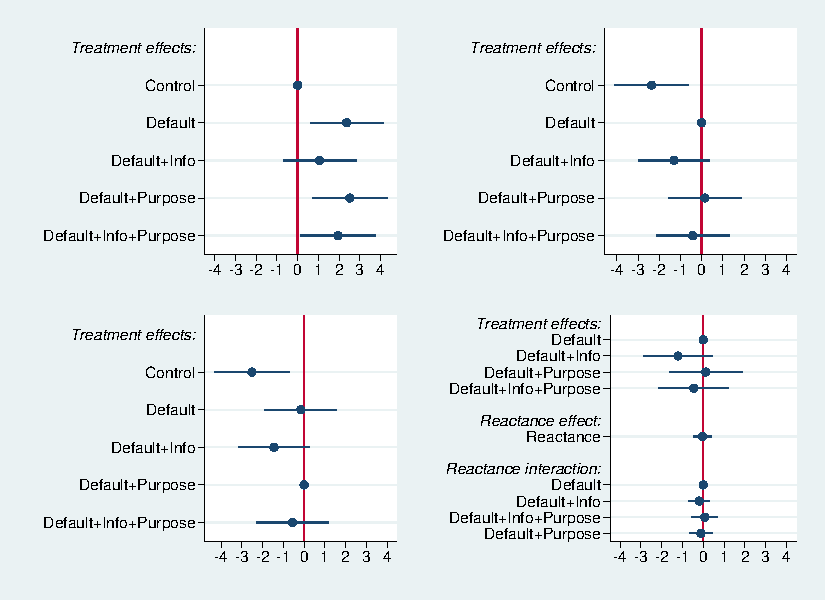
\includegraphics[page=1,width=1\textwidth]{FigureB5}
  \label{figb5}
  \floatfoot{Notes: Dots with horizontal lines indicate point estimates with 95\% confidence intervals from Tobit models. Dots on the zero line denote the reference category. Models (3) and (8) in Tables~\ref{tab4} and ~\ref{tab6} display the underlying regression results. The top left panel refers to finding F1, the top right panel to F2 and F3, the bottom left panel to F4, and the panel on the bottom right to F6. Covariates are not shown.}
  \end{tabular}
\end{figure}

\begin{figure}[h]
\caption{Default and transparency effects on perceived Threat to freedom}
   \centering
   \begin{tabular}{@{}c@{\hspace{.5cm}}c@{}}
       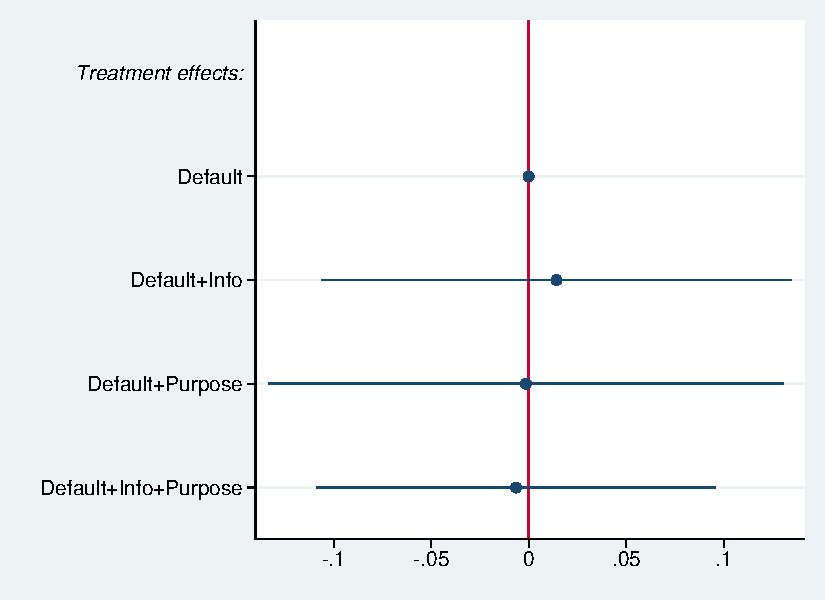
\includegraphics[page=1,width=0.6\textwidth]{FigureB6}
  \label{figb6}
  \floatfoot{Notes: Dots with horizontal lines indicate point estimates with 95\% confidence intervals from marginal effects of ordered logistic models. Dots on the zero line denote the reference category. Model (4) in Table~\ref{tab5} displays the underlying regression results (albeit not showing marginal effects). It refers to finding F5. Covariates are not shown.}
  \end{tabular}
\end{figure}

\begin{figure}[h]
\caption{Default and transparency effects on Anger}
   \centering
   \begin{tabular}{@{}c@{\hspace{.5cm}}c@{}}
       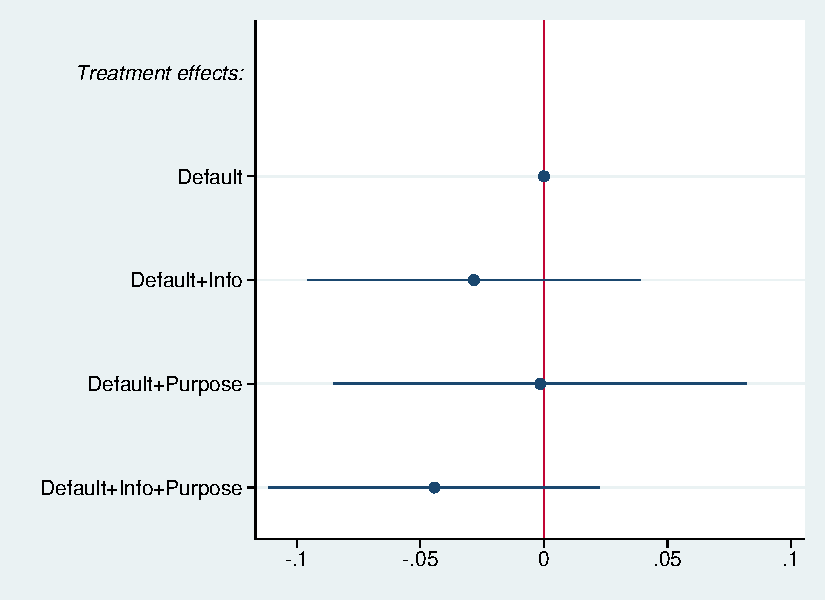
\includegraphics[page=1,width=0.6\textwidth]{FigureB7}
  \label{figb7}
  \floatfoot{Notes: Dots with horizontal lines indicate point estimates with 95\% confidence intervals from marginal effects of ordered logistic models. Dots on the zero line denote the reference category. Model (5) in Table~\ref{tab5} displays the underlying regression results (albeit not showing marginal effects). It refers to finding F5. Covariates are not shown.}
  \end{tabular}
\end{figure}

\clearpage

\section{Questionnaire} 
\label{appc}

\textbf{Questionnaire on covariates} \\
\\
What is you gender? O Male O Female \\
\\
What is your age? \\
\\
Have you participated in other experiments before today? O Yes O No \\
\\
How important is climate protection for you? Please circle the most suitable answer. \\
O Not important at all O Not important O Indifferent O Important O Very important\\
\\
Do you think that buying real carbon dioxide (CO$_2$) emissions licenses on the market of the European Union Emissions Trading Scheme (EU ETS) is an effective method to contribute to climate protection? O Yes O No \\
\\
\textbf{Questionnaire on state reactance} \\

Please indicate to what extent do you agree with the following statements on a 5-point response scale that ranges from the statement – "strongly disagree" to the statement – "strongly agree". (Perceived threat to freedom)\\

\begin{itemize}
\item The default value threatened my freedom to choose.
\item The default value tried to make a decision for me.
\item The default value tried to manipulate me.
\item The default value tried to pressure me.
\end{itemize}

Please indicate to what extent do you agree with the following statements on a 5-point response scale that ranges from the statement – "Not at all" to the statement – "Very". (anger) \\

\begin{itemize}
\item Please indicate how irritated you were with regard to the given default value.
\item Please indicate how angry you were with regard to the given default value.
\item Please indicate how annoyed you were with regard to the given default value.
\item Please indicate how aggravated you were with regard to the given default value. \\
\end{itemize}


\textbf{Questionnaire on trait reactance} \\

Please indicate to what extent do you agree with the following statements on a p-point response scale that ranges from the statement – "strongly disagree" to the statement – "strongly agree". \\

\begin{itemize}
\item Regulations trigger a sense of resistance in me.
\item I find contradicting others stimulating.
\item When something is prohibited, I usually think, "that's exactly what I am going to do".
\item The thought of being dependent on others aggravates me.
\item I consider advice from others to be an intrusion.
\item I become frustrated when I am unable to make free and independent decisions.
\item It irritates me when someone points out things, which are obvious to me.
\item I become angry when my freedom of choice is restricted.
\item Advice and recommendations usually induce me to do just the opposite.
\item I am content only when I am acting on my own free will.
\item I resist the attempts of others to influence me.
\item It makes me angry when another person is held up as a role model for me to follow.
\item When someone forces me to do something, I feel like doing the opposite.
\item It disappoints me to see others submitting to standards and rules.
\end{itemize}


\end{document}

%%
%% End of file `elsarticle-template-2-harv.tex'.
